\documentclass[10pt,a4paper]{report}
\usepackage[utf8]{inputenc}
\usepackage[french]{babel}
\shorthandoff{;:!?} % désactive les caractères actifs de babel-french pour garder la mise en page identique
\usepackage[T1]{fontenc}
\usepackage{amsmath}
\usepackage{amsfonts}
\usepackage{amssymb}
\usepackage{makeidx}
\usepackage[pdftex]{graphicx}
\usepackage{lmodern}
\usepackage{kpfonts}
%\usepackage{fourier}
\usepackage{multicol,caption}
\usepackage{float}
\usepackage{listings}
\usepackage{xcolor}
\usepackage{ifthen}
\usepackage{etoolbox}
\usepackage{lastpage}
\usepackage{fancyhdr}
\usepackage{lipsum}
\usepackage{appendix}
\usepackage[left=2cm,right=2cm,top=3cm,bottom=4cm, headsep=55pt, , inner=2.5cm, outer=1.5cm]{geometry}
\usepackage[skip=10pt plus1pt, indent=0pt]{parskip}
\usepackage{array}
\usepackage{tabularx}
\usepackage{tabularray}
\usepackage{tocloft}
\usepackage{tikz}
\usepackage{tikz-cd}
\usepackage{physics} % Pour \vb (vecteurs en gras)
\usetikzlibrary{positioning,fit,shapes.geometric,arrows.meta, positioning, matrix}
\usepackage{amsmath} % Pour \mathbf et \hat

\usepackage{calrsfs}
\DeclareMathAlphabet{\pazocal}{OMS}{zplm}{m}{n}


\tikzset{
   actor/.style={
     circle,
     draw=black,
     minimum size=3mm
   },
   arrow/.style={
     -latex,
     thick,
     shorten <=2pt,
     shorten >=2pt
   },
   column/.style={
   -latex,
   sep=-6ex, 
   row sep=1ex
   }
}

%%gmedina solution
\newcommand{\listequationsname}{Liste des équations}
\newlistof{myequations}{equ}{\listequationsname}
\newcommand{\myequations}[1]{%
\addcontentsline{equ}{myequations}{\protect\numberline{\theequation}#1}\par}
\setlength{\cftmyequationsnumwidth}{2.5em}% Width of equation number in List of Equations


\newcommand{\listremarksname}{Liste des remarques}
\newlistof{myremarks}{rmk}{\listremarksname}
\newcounter{rmkcntr}
\newcommand{\myremarks}[2]{%
\stepcounter{rmkcntr}%
\addcontentsline{rmk}{myremarks}{\protect\numberline{\thermkcntr}#1}\par\fbox{%
\begin{minipage}[c]{0.3\textwidth}
\textit{\textbf{Remarque \thermkcntr : #1 }}
\end{minipage}%
\vrule\enskip\vrule\quad
\begin{minipage}{\dimexpr 0.7\textwidth-0.8pt-1.5em}
\textit{#2} 
%\label{rq:rq0}
\end{minipage} \\
}}
\setlength{\cftmyremarksnumwidth}{2.5em}% Width of remark number in List of remarks



\newcommand{\listdefinitionsname}{Liste des définitions}
\newlistof{mydefinitions}{def}{\listdefinitionsname}
\newcounter{defcntr}
\newcommand{\mydefinitions}[2]{%
\stepcounter{defcntr}%
\addcontentsline{def}{mydefinitions}{\protect\numberline{\thedefcntr}#1}\par\fbox{%
\begin{minipage}[c]{0.3\textwidth}
\textit{\textbf{Définition \thedefcntr : #1 }}
\end{minipage}%
\vrule\enskip\vrule\quad
\begin{minipage}{\dimexpr 0.7\textwidth-0.8pt-1.5em}
\textit{#2} 
%\label{rq:rq0}
\end{minipage} \\
}}
\setlength{\cftmydefinitionsnumwidth}{2.5em}% Width of definition number in List of definitions



\pagestyle{headings}
% definition paragaph en subsubsubsection
\setcounter{secnumdepth}{5}
\setcounter{tocdepth}{5}
\makeatletter
\newcommand\subsubsubsection{\@startsection{paragraph}{4}{\z@}{-2.5ex\@plus -1ex \@minus -.25ex}{1.25ex \@plus .25ex}{\normalfont\normalsize\bfseries}}
\newcommand\subsubsubsubsection{\@startsection{subparagraph}{5}{\z@}{-2.5ex\@plus -1ex \@minus -.25ex}{1.25ex \@plus .25ex}{\normalfont\normalsize\bfseries}}
\makeatother

\definecolor{codegreen}{rgb}{0,0.6,0}
\definecolor{codegray}{rgb}{0.5,0.5,0.5}
\definecolor{codepurple}{rgb}{0.58,0,0.82}
\definecolor{backcolour}{rgb}{0.95,0.95,0.92}

\lstdefinestyle{mystyle}{
    backgroundcolor=\color{backcolour},   
    commentstyle=\color{codegreen},
    keywordstyle=\color{magenta},
    numberstyle=\tiny\color{codegray},
    stringstyle=\color{codepurple},
    basicstyle=\ttfamily\fontsize{8pt}{8pt}\selectfont,
    breakatwhitespace=false,         
    breaklines=true,                 
    captionpos=b,                    
    keepspaces=true,                 
    numbers=left,                    
    numbersep=5pt,                  
    showspaces=false,                
    showstringspaces=false,
    showtabs=false,                  
    tabsize=5
}

\renewcommand{\chaptermark}[1]{\markboth{#1}{#1}}
\fancypagestyle{plain}{
\fancyhf{}% Clear header/footer
\renewcommand{\headrulewidth}{1pt}
\fancyhead[RO,RE]{ Simulateur de Golf en Scilab v0.1}
\fancyhead[CO,CE]{\textcolor{red}{free}}
\fancyhead[LO,LE]{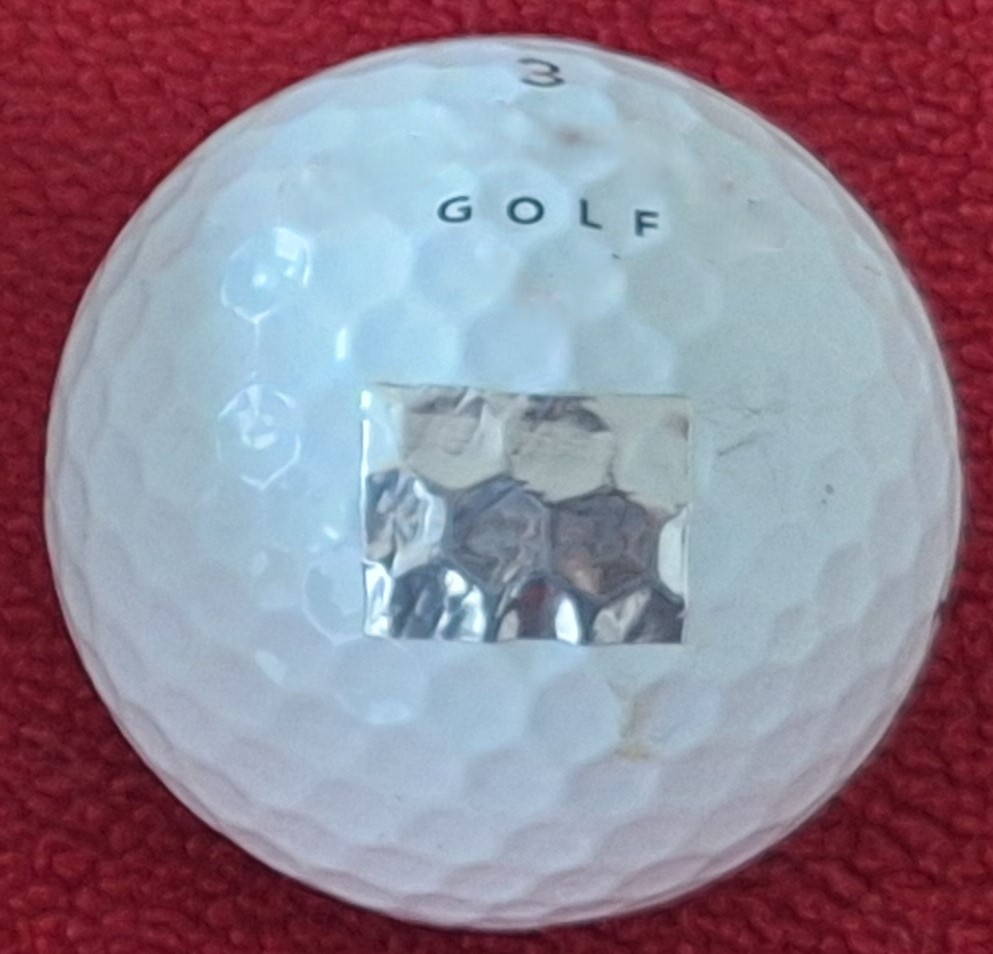
\includegraphics[width=0.5cm]{Logo-golfball.jpg}}
\fancyfoot[LO,CE]{\fontsize{8}{11}\selectfont\textit{\begin{center}Ce document et les informations qu'il contient sont la propriété de Matthieu PHILIPPE.\\Ils ne doivent être ni copiés ni divulgués à des tiers sans autorisation écrite préalable.\end{center}}\begin{flushright} \end{flushright}}
}

\fancypagestyle{plain2}{
\fancyhf{}% Clear header/footer
\renewcommand{\headrulewidth}{0pt}
\fancyhead[LO,LE]{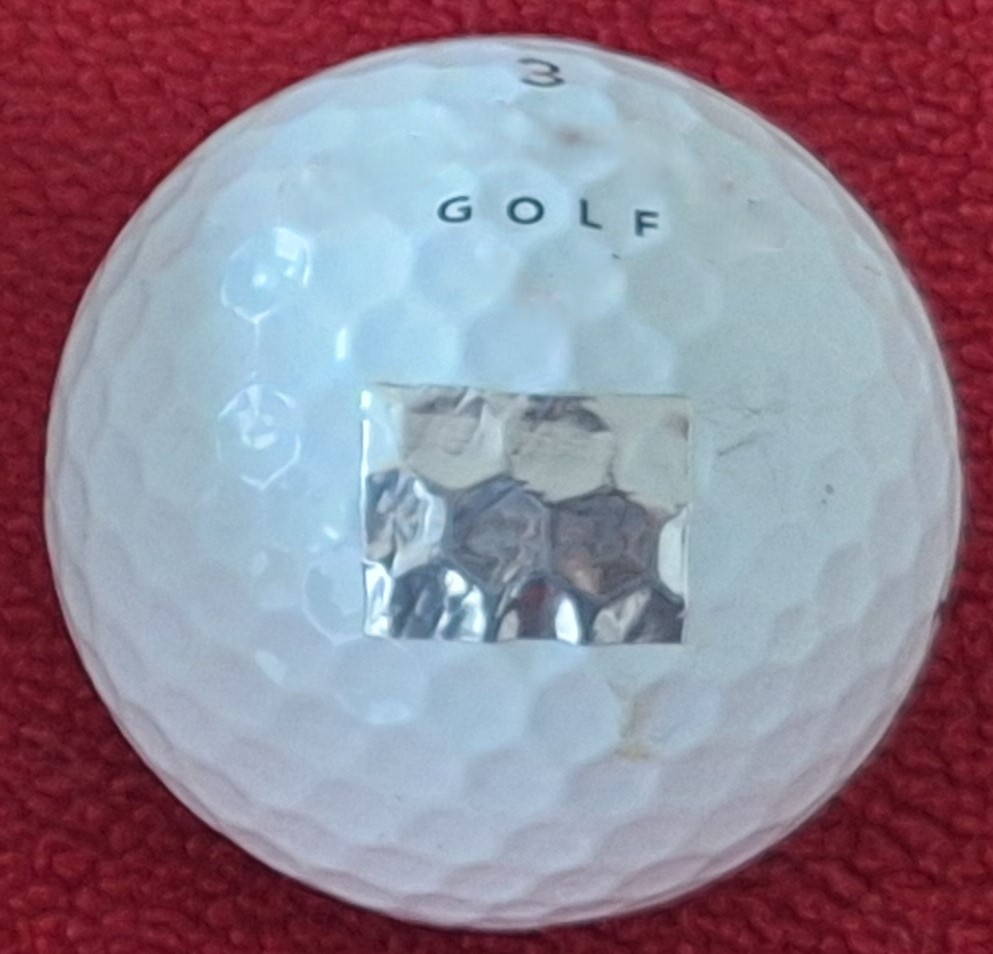
\includegraphics[width=0.5cm]{Logo-golfball.jpg}}
\fancyhead[RO,RE]{ }
\fancyhead[CO,CE]{\textcolor{red}{free}}
\fancyfoot[LO,CE]{\fontsize{8}{11}\selectfont\textit{\begin{center}This document and the information contained herein are the property of Matthieu PHILIPPE.\\They must not be copied or disclosed to third parties without prior written authorization.\end{center}}\begin{flushright}-\end{flushright}}
}

\fancypagestyle{plainstar}{
\fancyhf{}% Clear header/footer
\renewcommand{\headrulewidth}{1pt}
\fancyhead[LO,LE]{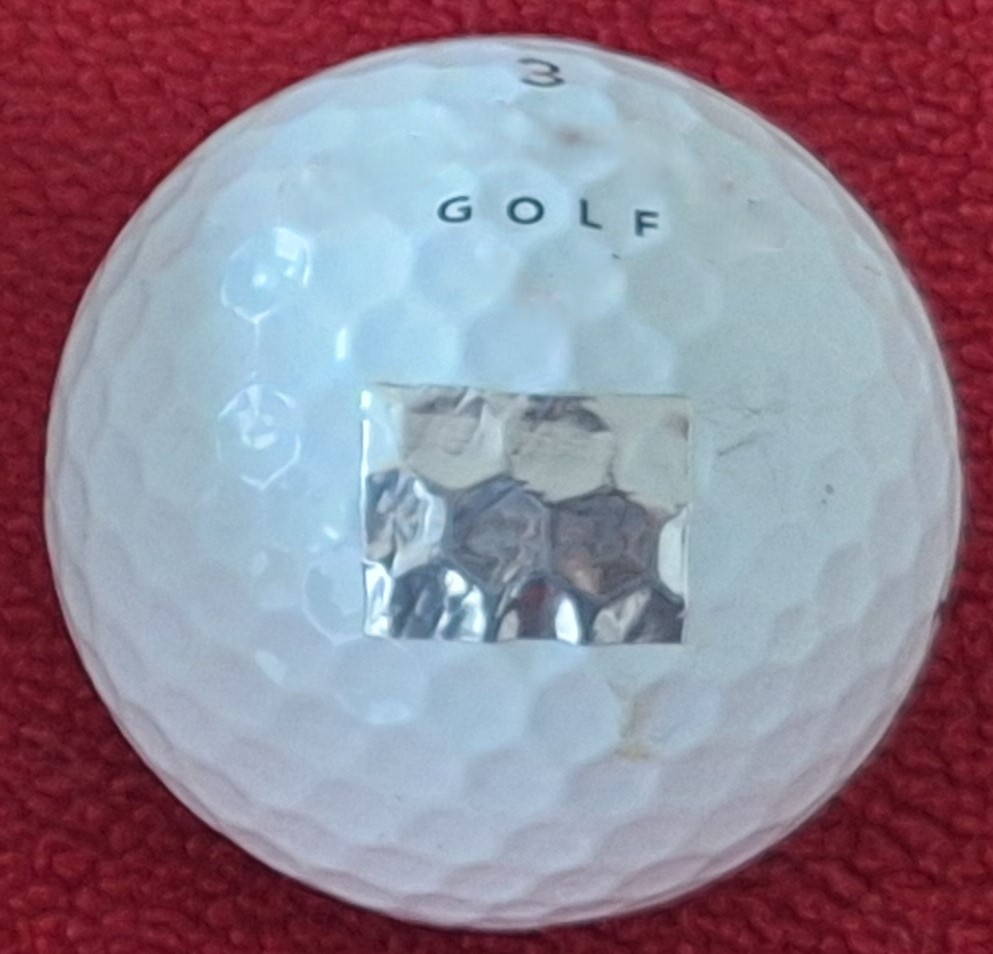
\includegraphics[width=0.5cm]{Logo-golfball.jpg}}
\fancyhead[RO,RE]{Page \thepage\  / \pageref{LastPage} }
\fancyhead[CO,CE]{\textcolor{red}{free}}
\fancyfoot[LO,CE]{\fontsize{8}{11}\selectfont\textit{\begin{center}This document and the information contained herein are the property of Matthieu PHILIPPE.\\They must not be copied or disclosed to third parties without prior written authorization.\end{center}}\begin{flushright}-\end{flushright}}
}



\fancypagestyle{noheader}{
\fancyhf{}% Clear header/footer
\fancyhead[LO,LE]{}
\fancyhead[CO,CE]{\textcolor{red}{free}}
\fancyhead[RO,RE]{}
}

\lstset{style=mystyle}

\usepackage[left=2cm,right=2cm,top=3cm,bottom=4cm, headsep=55pt]{geometry}

\author{Matthieu PHILIPPE\\Publication Perso}

\title{\textbf{Simulateur de Golf en Scilab :\\Capture d'un swing et estimation de la portée\\avec un petit radar low-cost}}

\begin{document}
\sffamily
%\pagestyle{plain}

\rmfamily\maketitle\sffamily
%\noindent\makebox[\linewidth]{\rule{\textwidth}{0.4pt}}
\tableofcontents
\listoffigures
\listoftables
\lstlistoflistings
\listofmyequations
\listofmyremarks
\listofmydefinitions

\newpage
\pagestyle{plainstar}
\section*{RÉSUMÉ}\setcounter{page}{1}
En utilisant les équations de la dynamique de vol d'une balle de golf, cet article montre comment coder un simulateur de swing de balle en Scilab.

Le simulateur utilise un solveur d'EDO (équations différentielles ordinaires) de Scilab, les équations de la dynamique des fluides appliquées à une balle (gravité, traînée, forces de Magnus), la restitution des forces d'un club de golf appliquée à une balle pour les départs, son vol, ses rebonds et son roulement. 

Dans la seconde partie, l'article présente une méthode pour capturer la vitesse de la balle en vol à l'aide de 2 radars low-cost, couplés à un Arduino Mini et une carte son adaptée connectée à la sortie du radar. 

Le signal radar est enregistré au format WAV puis filtré pour extraire vitesse et spin pendant les premiers mètres de vol, en utilisant la densité spectrale de puissance en mode temps réel.

\emph{\textbf{Mots-clés :} Balle de golf, Simulateur, Scilab, Radar, Densité spectrale.}

\chapter{Introduction}
Après quelques années à jouer au golf, j'ai voulu en savoir plus sur la dynamique des interactions entre le club, la balle et les éléments. 

Bien sûr, la littérature académique et les publications étaient assez abondantes. Mais je suis tombé sur des articles \cite{PWBJKH76} de 1976 et \cite{SASDR94} de 1994. La description de la physique de la balle m'a poussé à modéliser ce système en Scilab (fig \ref{fig:hmisimulation}). Ensuite, je l'ai fait en Java, C++, puis C\# pour l'utiliser sous \emph{Unity game engine}{\textregistered \texttrademark}.


\begin{figure} [H]\centering
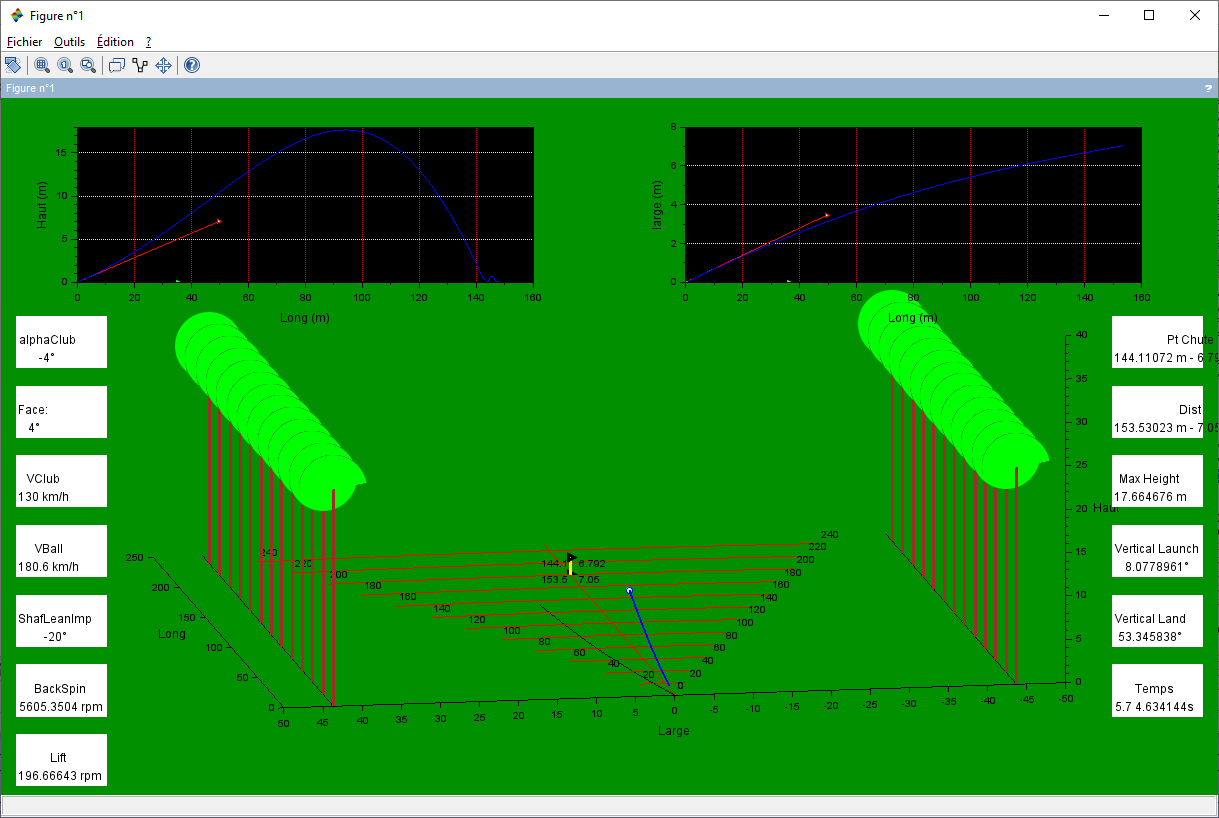
\includegraphics[width=10cm,keepaspectratio, ]{../sci/img/Pasted image 20250120171635.png}
\caption{IHM de la simulation}
\label{fig:hmisimulation}
\end{figure}


Quand les résultats ont été satisfaisants, j'ai pensé à capturer le vol d'une balle de golf avec de l'instrumentation. Après des essais au sonar, largement insuffisants, j'ai pris de petits radars de détection de présence pour portes automatiques.

Je ne savais pas dans quoi je m'engageais, mais après avoir remis à jour mes connaissances en filtrage du signal et quelques lignes de programmation en Scilab, j'ai trouvé un moyen de capturer les données essentielles : la vitesse et le backspin de la balle en vol, ainsi que l'écho du club juste avant l'impact et pendant le vol (fig \ref{fig:radarcapture0}).

\begin{figure} [H]\centering
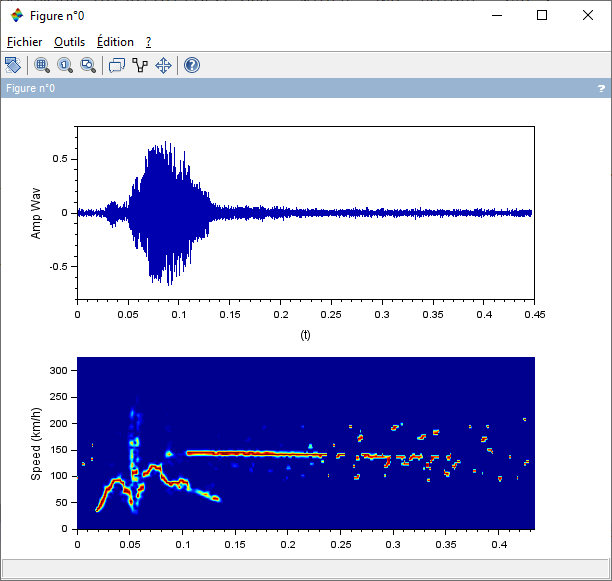
\includegraphics[width=8cm,keepaspectratio, ]{../sci/img/Pasted image 20250122083320.png}
\caption{Captures radar}
\label{fig:radarcapture0}
\end{figure}

Cet article décrit tout ce que j'ai trouvé et comment j'ai assemblé le tout : équations, programmes, filtrage, estimateurs et composants électroniques pour réaliser une simulation virtuelle de golf.

Toutes les équations présentées dans cet article sont issues de publications ou d'ouvrages publics, référencés dans la bibliographie. Je ne reviendrai pas sur les démonstrations et explications physiques, qui ne sont pas l'objet de ces pages. Ce qui m'importe, c'est le lien entre ces informations et la façon dont je les ai utilisées ou adaptées.

\chapter{Vol de la balle de golf}

L'équation principale est celle du vol de la balle. Elle rend compte de 3 forces : la force de Magnus, la traînée de l'air et la gravité, telles que :

\begin{equation}\label{eq:flightforces}
\sum{\overrightarrow{F}} =  \overrightarrow{F_{m}} + \overrightarrow{F_{d}} + \overrightarrow{F_{g}}
\end{equation}\myequations{Forces en vol}

\bigskip
\begin{figure}[h]
\centering
\label{fig:forces_golf_ball}
\begin{tikzpicture}[
    scale=1.5,
    force/.style={->, thick, line cap=round},
    velocity/.style={->, thick, blue, line cap=round},
    spin/.style={->, thick, purple, line cap=round},
    axis/.style={->, gray, thin},
    node distance=0.5cm and 1cm,
]

% --- Draw the golf ball (as a circle) ---
\draw[fill=white, draw=black, thick] (0,0) circle (0.5cm);

% --- Draw velocity vector (v) ---
\draw[velocity] (0,0) -- (1.5,0.5) node[right] {$\mathbf{v}$};

% --- Draw spin vector (omega) ---
\draw[spin] (0,0) -- (-0.3,0.8) node[above left] {$\mathbf{\omega}$};

% --- Draw forces ---
% Drag force (opposite to velocity)
\draw[force, red] (0,0) -- (-0.8,-0.3) node[left] {$\mathbf{F}_D$};

% Magnus force (perpendicular to v and omega)
\draw[force, green!60!black] (0,0) -- (0,1.2) node[above] {$\mathbf{F}_M$};

% Gravity force (downwards)
\draw[force, orange] (0,0) -- (0,-1.2) node[below] {$\mathbf{F}_g$};

% --- Draw coordinate system ---
\draw[axis] (0,0) -- (2,0) node[right] {$x$};
\draw[axis] (0,0) -- (0,2) node[above] {$y$};
\draw[axis] (0,0) -- (-1.5,-1) node[below left] {$z$};

% --- Add right-hand rule for spin ---
\draw[->, purple, dashed] (-0.3,0.8) arc (120:180:0.5) node[left] {$\omega$};
\draw[->, purple, dashed] (0,0) -- (-0.5,0) node[left] {$\hat{\mathbf{x}}$};
\draw[->, purple, dashed] (0,0) -- (0,0.5) node[above] {$\hat{\mathbf{y}}$};

% --- Add legend ---
\matrix[draw, below left=1cm and -1cm of current bounding box.south east, anchor=north east] {
    \draw[velocity] (0,0) -- (0.5,0); & \node[right] {Vitesse $\mathbf{v}$}; \\
    \draw[force, red] (0,0) -- (0.5,0); & \node[right] {Traînée $\mathbf{F}_D$}; \\
    \draw[force, green!60!black] (0,0) -- (0.5,0); & \node[right] {Portance $\mathbf{F}_M$}; \\
    \draw[force, orange] (0,0) -- (0.5,0); & \node[right] {Gravité $\mathbf{F}_g$}; \\
    \draw[spin] (0,0) -- (0.5,0); & \node[right] {Spin $\mathbf{\omega}$}; \\
};

\end{tikzpicture}
\caption{\textbf{Schéma des forces agissant sur une balle de golf en vol.}}

\end{figure}


\bigskip
\section{Force de traînée}
\subsection{Caractéristiques de l'air}

\mydefinitions{Force de traînée de l'air}{La force de traînée de l'air est la résistance s'exerçant sur la section droite d'un objet, orthogonale au déplacement, déterminée par la relation donnée par \cite{BBRS11} (\ref{eq:aircaracteristic2})} :

\begin{eqnarray}
F_d(V)&=&-\frac{1}{2}.\rho(T).C_d.S.V^2(t)\label{eq:aircaracteristic2}
\end{eqnarray}\myequations{Résistance de l'air}

où :
\begin{eqnarray*}\label{eq:aircaracteristiccst}
\rho(T)&=&1,292*\frac{273,15}{273,15+ T}\label{eq:aircaracteristic1}\\
\rho(T)\ &=&densité\ de\ l'air\ \rho\ selon\ la\ température\ T\\
T&=&Température\\
C_d\ &=&Coefficient\ de\ traînée,\ dépendant\ de\ l'objet\\
V&=&Vitesse\ de\ l'objet\\
F_d(V)\ &=&Force\ de\ traînée\ due\ à\ la\ résistance\ de\ l'air,\ selon\ la\ vitesse\ V\\
S&=& Section\ droite\ exposée,\ orthogonale\ au\ déplacement.
\end{eqnarray*}

\subsection{Caractéristiques de la balle dans l'air}

En considérant ces caractéristiques d'un modèle de balle alvéolée,

\begin{eqnarray*}\label{eq:massdiameterintertia}
mass\ m&=&0,04593\ g \\
Dynamic\ viscosity\ \mu&=&1,5.10^{-6} m^2/s\\
Diameter\ D&=&0,04267\ m\\
Radius\ r&=&\frac{D}{2}\\
Inertia\ I&=&\frac{2}{5}.m.R^2\\
Cross-section\  S&=&\pi.R^2\\
Ball\ Velocity\ &=&V
\end{eqnarray*}\myequations{Masse, diamètre, rayon, inertie, section, nombre de Reynolds}

Nous avons un modèle estimé,

\begin{eqnarray}\label{eq:dragforce}
Re&=&\frac{\rho(T).V.D}{\mu}\label{eq:reynoldsnb}\\
C_d&=&0,36 + \frac{24}{Re} + \frac{6}{1+\sqrt{Re}}\label{eq:dragforce4}\\
\overrightarrow{F_{d}} &=& -\frac{1}{2}.\rho(T).C_d.S.\sqrt{(V(x)^2+V(y)^2+V(z)^2)}.\widehat{V}
\end{eqnarray}\myequations{Coefficient de traînée, force de traînée}

où :

\begin{eqnarray*}\label{eq:dragforce2}
\widehat{V}&=&Vecteur\ unitaire\ de\ la\ vitesse\\
Re&=&Estimateur\ du\ nombre\ de\ Reynolds\\
C_d&=&Coefficient\ de\ traînée,\ relation\ de\ White\\
\overrightarrow{F_{d}}&=& Force\ de\ traînée
\end{eqnarray*}


\myremarks{Enfin, l'équation de la force de traînée selon les 3 axes devient \ref{eq:vectordragforce}}{\begin{equation}\label{eq:vectordragforce}
\overrightarrow{F_d} = \begin{pmatrix}
-\frac{1}{2}.\rho(T).C_d.S.v_{i}^2 \\
-\frac{1}{2}.\rho(T).C_d.S.v_{j}^2 \\
-\frac{1}{2}.\rho(T).C_d.S.v_{k}^2
\end{pmatrix}
\end{equation}
}

\section{Effet Magnus}
\mydefinitions{Effet Magnus}{L'effet Magnus \cite{magnus1853abweichung} est dû à la rotation d'un objet cylindrique se déplaçant dans un fluide (l'air). On l'appelle effet Robin pour une balle.} 

Par généralisation, le nom d'effet Magnus est appliqué à tout objet soumis à cette force d'aspiration. Cette force de portance apparaît et modifie la trajectoire balistique de la balle de golf. La force dépend du coefficient de portance (\emph{$C_l$}), associé à l'objet selon sa forme, sa nature et sa texture. La force s'écrit donc comme une composante de la vitesse de l'objet, du taux de spin et d'un coefficient d'effet Magnus \emph{$C_m$} (\ref{eq:magnusforce1}),


\begin{eqnarray}\label{eq:magnusforce}
\overrightarrow{F_{m}} &=& C_m.(\overrightarrow{\omega}\ \times\  \overrightarrow{V})\label{eq:magnusforce1}
\end{eqnarray}\myequations{Effet de portance Magnus}


où :
\begin{eqnarray*}\label{eq:dragforce3}
\omega&=&spin\ en\ rad/s\\
V_p&=&r\omega\ vitesse\ périphérique\\
V&=&Vitesse\ de\ la\ balle\\
C_m&=&Coefficient\ d'effet\ Magnus
\end{eqnarray*}

La bibliographie principale que j'ai utilisée pour la balle de golf est \cite{GPA05} et \cite{SASDR94}. J'ai trouvé plusieurs façons de calculer le $C_m$, données ci-dessous. La première approximation simple est donnée par \ref{eq:magnusforce2}, et le coefficient d'effet Magnus peut être donné par les deux premiers estimateurs ci-dessous \ref{eq:magnusforce3}, \ref{eq:magnusforce4} (\cite{GPA05}). Mais j'ai retenu celui-ci \ref{eq:magnusforce5} (\cite{SASDR94}, \cite{AL98}). 

\begin{eqnarray}\label{eq:magnusforce0}
F_m&=& \frac{1}{2}.C_m.\rho.\mu^2\label{eq:magnusforce2}\\
C_m&=&\frac{r\omega}{V}\label{eq:magnusforce3}\\
C_m&=&-0,05+ \sqrt{0,0025 + 0,36\left( \frac{r\omega}{V}\right)}\label{eq:magnusforce4}\\
C_m &=&0,5 . \rho(T). S. R^2. C_l.\mid{\frac{\omega}{V}}\mid^{0,4}.V\label{eq:magnusforce5}\\
C_l&=&\frac{1}{2 + (V/R\omega)*sin(\zeta)}\label{eq:magnusforce6}
\end{eqnarray}\myequations{Effet Magnus et différents modèles de coefficient}

\cite{GGA} donne un coefficient de correction $C_{l}$ (\ref{eq:magnusforce6}) à appliquer à (\ref{eq:magnusforce5}), où $\zeta$, dans le coefficient de portance, est l'angle entre l'axe de rotation et la direction du mouvement. Si R$\omega\ll$ V, alors $C_l \simeq R\omega \frac{sin\zeta}{V}$. Certainement plus approprié que (\ref{eq:magnusforce3}) pour prendre en compte l'effet du spin latéral et du backspin.

\begin{eqnarray}\label{eq:zeta}
sin\zeta = \frac{\parallel\overrightarrow{\omega} \times \overrightarrow{V}\parallel}{\omega.V} = \frac{1}{\omega.V}.\sqrt{((\omega_j.V_k -\omega_k.V_j )^2 + ( \omega_k.V_i -\omega_i.V_k )^2 +( \omega_i.V_j -\omega_j.V_i )^2)}
\end{eqnarray}\myequations{Angle entre axes de mouvement et de spin}

Pour répondre à mes besoins, j'ai choisi de fournir mes valeurs adaptées de $C_l$ à (\ref{eq:magnusforce5}) plutôt que (\ref{eq:magnusforce6}), issues de tests avec mes propres balles (la texture et le nombre d'alvéoles jouent sur le nombre de Reynolds (\ref{eq:reynoldsnb}) comme montré dans \cite{ASCM11}). Ces données sont enregistrées dans une table Scilab $C_{l1}$. $C_m$ devient (\ref{eq:magnusforce7}). 
\begin{eqnarray}
C_m &=&0,5 . \rho(T). S. R^2. C_{l1}.\mid{\frac{\omega}{V}}\mid^{0,4}.V\label{eq:magnusforce7}
\end{eqnarray}
Mes propres $C_{l1}$ pour les clubs Mizuno JPX et la balle Decathlon sont données en exemple dans le tableau \ref{eq:mycl1}.

\begin{table}[h!]
\centering
\begin{tabular}{|c|c|}
\hline
\textbf{Club} & \textbf{$C_{l1}$} \\
\hline
D & 0.64 \\
W5 & 0.65 \\
H3 & 0.54 \\
I5 & 0.54 \\
I6 & 0.83 \\
I7 & 0.42 \\
I8 & 0.53 \\
I9 & 0.53 \\
PW & 0.52 \\
AW & 0.52 \\
SW & 0.51 \\
LW & 0.51 \\
\hline
\end{tabular}
\caption{Table de mes $C_{l1}$}
\label{eq:mycl1}
\end{table}

\myremarks{Connaissant \ref{eq:magnusforce1}, \ref{eq:magnusforce7} et \ref{eq:mycl1}, j'ai choisi le modèle de force de Magnus suivant}{\begin{equation}\label{eq:vectormagnusforce}
\overrightarrow{F_m} = \begin{pmatrix}
C_m*(\omega_j*v_k-\omega_k*v_j) \\
C_m*(\omega_k*v_i-\omega_i*v_k) \\
C_m*(\omega_i*v_j-\omega_j*v_i)
\end{pmatrix}
\end{equation}
}

\section{Force de gravité}
\mydefinitions{La force de gravité}{La force de gravité est déterminée par l'accélération \emph{g} vers le sol.}

L'expression de la force de gravité est simplement,
\myremarks{La force de gravité}{\begin{equation}\label{eq:vectorgravityforce}
\overrightarrow{F_g} = \begin{pmatrix}
0\\
-mg\\
0
 \end{pmatrix}
\end{equation}\myequations{Force de gravité}
}


\section{Vitesse de départ}
Par l'impact du club de golf sur la balle, il résulte un vol de balle avec un angle de départ. Le loft de la tête de club détermine l'angle de départ ; la vitesse de la tête de club et la texture des deux déterminent la vitesse de balle au départ et le spin de la balle \cite{PA01}.

À cause de la texture, il y a une perte d'énergie, que l'on peut prendre en compte via le coefficient de restitution \emph{e} (COR \cite{BLSJ94}).

\begin{figure} [H]\centering
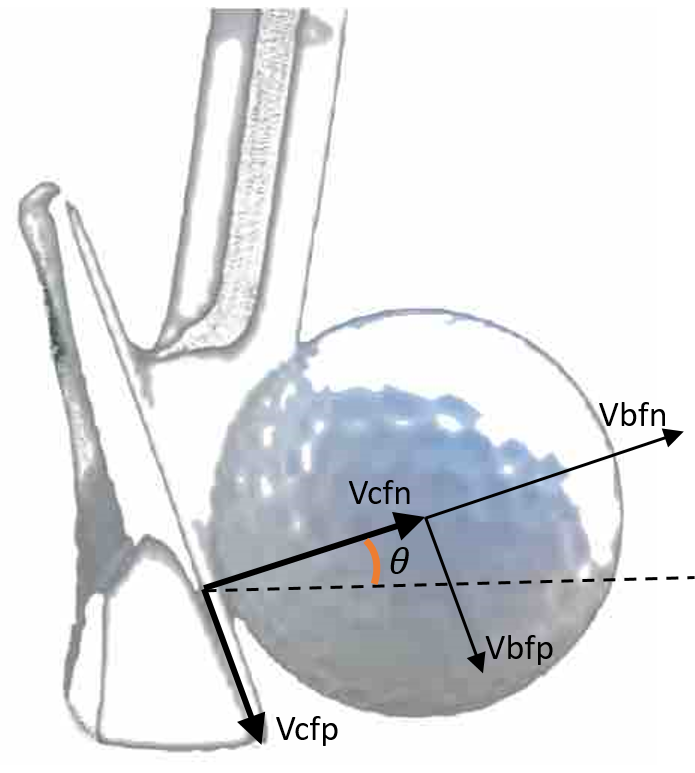
\includegraphics[width=6cm,keepaspectratio, ]{ImpactClubBall.png}
\caption{Composantes de vitesse}
\label{fig:impactclubball}
\end{figure}


\cite{PA01} donne une estimation du COR e : 
\begin{eqnarray}
e&=&0,86\ -\ 0,0029.V_{ci}.cos(\theta)\\
V_{bfn}&=&V_{ci}.cos(\theta).\frac{1+e}{1+\frac{m}{M}}\\
V_{bfp}&=&-V_{ci}.\frac{sin(\theta)}{1+\frac{m}{M} + \frac{5}{2}}\\
\psi_{bo}&=&\theta + \arctan\left(\frac{V_{bfp}}{V_{bfn}}\right)\\
\omega_{bo}&=&\omega_{bf} = -m.V_{bfp}.\frac{R}{I}
\end{eqnarray}\myequations{Vitesse de la balle et angle de départ après l'impact du club}


où :
\begin{eqnarray*}
V_{ci}&=&Vitesse\ initiale\ du\ club,\ parallèle\ au\ sol.\\
V_{bfn}&=&Vitesse\ finale\ de\ la\ balle\ orthogonale\ à\ la\ face\ du\ club\\
V_{bfp}&=&Vitesse\ de\ la\ balle\ de\ golf,\ parallèle\ à\ la\ face\ du\ club\\
\theta&=&loft\ dynamique\ (\ loft\ du\ club + inclinaison\ du\ shaft\ à\ l'impact\ <\ loft)\\
e&=&COR,\ e\simeq0{,}78\ pour\ les\ fers,\ e\simeq0{,}83\ pour\ les\ drivers\ et\ les\ bois\\
\psi_{bo}&=&Angle\ de\ départ\\
\omega_{bo}&=&Spin\ de\ la\ balle\ de\ golf\\
I&=&Inertie\ (\ref{eq:massdiameterintertia})
\end{eqnarray*}

\section{Vitesse de la balle avec un centrage imparfait}
Il est difficile de centrer parfaitement la balle et le club. Le modèle de vitesse de balle est modifié pour inclure un paramètre \emph{Miss}. C'est l'écart au sweet spot ; la vitesse initiale de la balle dans ce cas est (\ref{eq.miss}),
\begin{equation}\label{eq.miss}
V_{bi}=(1-35.56*miss).\sqrt{V_{bfn}^2+V_{bfp}^2}\ (miss\ mesuré\ en\ mètre)
\end{equation}\myequations{Vitesse initiale de la balle après un centrage imparfait}

\section{Vitesse initiale de la face du club}
En fonction de la trajectoire du club ($\alpha_{cp}$) et de l'angle face/trajectoire ($\gamma_{fp}$), la vitesse initiale et le spin de la balle sont modifiés.

\begin{figure} [H]\centering
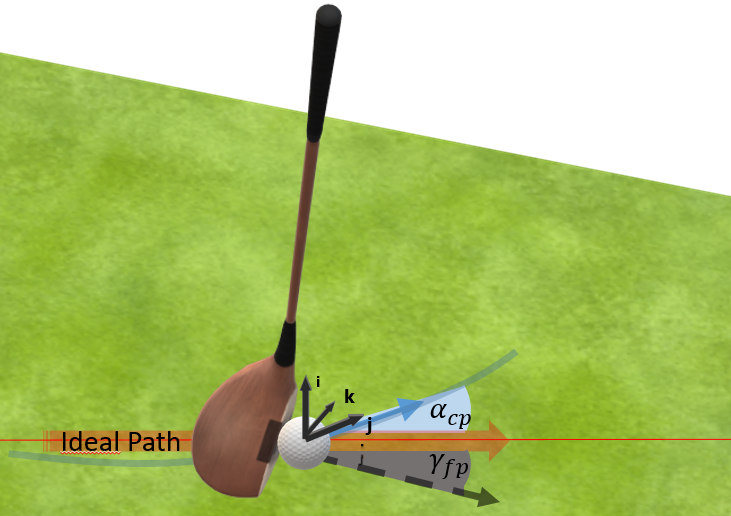
\includegraphics[width=12cm,keepaspectratio, ]{clubpath.png}
\caption{Trajectoire du club}
\label{fig:clubpath}
\end{figure}

Ainsi :

$V_{b0} \cdot \vb{i} = V_{bi} \cdot (1 - 0.3556 \cdot \text{miss}) \cdot \cos(\theta + \arctan(\frac{\sin(\theta) \cdot (1 + \frac{m}{M})}{(1 + e) \cdot \cos(\theta) \cdot (1 + \frac{m}{M} + \frac{5}{2})}))$
% Assurez-vous d'avoir ces packages dans votre préambule

$V_{b0} \cdot \overrightarrow{j} = V_{bi} \cdot (1 - 0.3556 \cdot \text{miss}) \cdot \sin\left(\theta + \arctan\left(\frac{\sin(\theta) \cdot \left(1 + \frac{m}{M}\right)}{(1 + e) \cdot \cos(\theta) \cdot \left(1 + \frac{m}{M} + \frac{5}{2}\right)}\right)\right)$

$V_{b0} \cdot \overrightarrow{k} = 0$

Le spin autour de l'axe $\overrightarrow{i}$ n'est pas une composante le long de l'axe de la trajectoire du club. Le spin s'applique dans le plan du sol, avec le \textit{SideSpin} aligné sur l'axe de la face du club $\overrightarrow{j}$, et le \textit{BackSpin} aligné sur l'axe de la trajectoire du club $\overrightarrow{k}$.
%
$w_{\overrightarrow{i}} = 0$

$w_{\overrightarrow{j}} = V_{b0} \cdot \overrightarrow{j} \cdot \sin(\alpha_{cp} - \gamma_{fp}) \cdot \text{Sac.coeffSpinLift}(\text{Sac.Type} == \text{Club})$

$w_{\overrightarrow{k}} = V_{b0} \cdot \overrightarrow{i} \cdot \sin(\theta) \cdot \text{Sac.coeffSpin}(\text{Sac.Type} == \text{Club})$

\section{Modèle complet de vol}
\subsection{Modèle complet de vol (forme matricielle/vectorielle)}
Le vol de la balle de golf est décrit par le système d'EDO suivant pour le vecteur d'état $\vec{Y} = \begin{pmatrix} x & y & z & V_x & V_y & V_z \end{pmatrix}^T$ :

\begin{equation}
    \frac{d\vec{Y}}{dt} = \begin{pmatrix}
    V_x \\
    V_y \\
    V_z \\
    -\frac{1}{2m} \rho(T) C_d S \|\vec{V}\| V_x + \frac{C_m}{m} (\omega_y V_z - \omega_z V_y) \\
    -\frac{1}{2m} \rho(T) C_d S \|\vec{V}\| V_y + \frac{C_m}{m} (\omega_z V_x - \omega_x V_z) - g \\
    -\frac{1}{2m} \rho(T) C_d S \|\vec{V}\| V_z + \frac{C_m}{m} (\omega_x V_y - \omega_y V_x)
    \end{pmatrix}
    \label{eq:ode_system}
\end{equation}

\noindent
où :
\begin{itemize}
    \item $\vec{V} = \begin{pmatrix} V_x \\ V_y \\ V_z \end{pmatrix}$ est le vecteur vitesse,
    \item $\vec{\omega} = \begin{pmatrix} \omega_x \\ \omega_y \\ \omega_z \end{pmatrix}$ est le vecteur spin,
    \item $\|\vec{V}\| = \sqrt{V_x^2 + V_y^2 + V_z^2}$ (norme),
    \item $C_d$ est le coefficient de traînée (équation~\ref{eq:dragforce4}),
    \item $C_m = 0.5 \rho(T) S R^2 C_{l1} \left( \frac{\|\vec{\omega}\|}{\|\vec{V}\|} \right)^{0.4} \|\vec{V}\|$ (équation~\ref{eq:magnusforce7}).
\end{itemize}

\subsubsection{Conditions initiales}
Le vecteur d'état initial $\vec{Y}_0$ est :
\begin{equation}
    \vec{Y}_0 = \begin{pmatrix}
    0 \\
    0 \\
    0 \\
    V_{bi} \cos\left( \theta + \arctan\left( \frac{\sin \theta \cdot (1 + \frac{m}{M})}{(1 + e) \cos \theta \cdot (1 + \frac{m}{M} + \frac{5}{2})} \right) \right) \\
    V_{bi} \sin\left( \theta + \arctan\left( \frac{\sin \theta \cdot (1 + \frac{m}{M})}{(1 + e) \cos \theta \cdot (1 + \frac{m}{M} + \frac{5}{2})} \right) \right) \\
    0
    \end{pmatrix}
    \label{eq:initial_conditions}
\end{equation}
avec $V_{bi} = (1 - 35.56 \cdot \text{miss}) \sqrt{V_{bfn}^2 + V_{bfp}^2}$ et $\vec{\omega}_0 = \begin{pmatrix} 0 & V_{b0y} \sin(\alpha_{cp} - \gamma_{fp}) \cdot \text{SpinLiftCoeff} & V_{b0x} \sin(\theta) \cdot \text{SpinCoeff} \end{pmatrix}^T$.

\subsection{Modèle complet de vol (notation tensorielle)}
La dynamique de vol de la balle de golf est décrite en notation tensorielle comme suit :

\subsubsection{Équation fondamentale}
L'évolution temporelle du vecteur d'état $\vec{Y} = \begin{pmatrix} \vec{r} \\ \vec{V} \end{pmatrix} \in \mathbb{R}^6$ est donnée par :
\begin{equation}
    \frac{d\vec{Y}}{dt} = \begin{pmatrix}
    \vec{V} \\
    \frac{1}{m} \left( \vec{F}_d + \vec{F}_m + \vec{F}_g \right)
    \end{pmatrix}
    \label{eq:tensor_ode}
\end{equation}

\subsubsection{Force de traînée}
La force de traînée est un champ vectoriel non linéaire :
\begin{equation}
    \vec{F}_d = -\frac{1}{2} \rho(T) \, C_d(\|\vec{V}\|, Re) \, S \, \|\vec{V}\| \, \vec{V}, \quad \|\vec{V}\| = \sqrt{\vec{V} \cdot \vec{V}}
    \label{eq:tensor_drag}
\end{equation}
où le coefficient de traînée $C_d$ dépend du nombre de Reynolds $Re = \frac{\rho(T) \|\vec{V}\| D}{\mu}$ :
\begin{equation}
    C_d = 0.36 + \frac{24}{Re} + \frac{6}{1 + \sqrt{Re}}.
    \label{eq:tensor_cd}
\end{equation}

\subsubsection{Force de Magnus}
La force de Magnus s'exprime à l'aide du produit vectoriel :
\begin{equation}
    \vec{F}_m = C_m \, (\vec{\omega} \times \vec{V}), \quad C_m = \frac{1}{2} \rho(T) \, S \, R^2 \, C_{l1} \, \left( \frac{\|\vec{\omega}\|}{\|\vec{V}\|} \right)^{0.4} \|\vec{V}\|
    \label{eq:tensor_magnus}
\end{equation}
où $\vec{\omega} \times \vec{V}$ est le produit vectoriel antisymétrique, représentable via le symbole de Levi-Civita $\epsilon_{ijk}$ :
\begin{equation}
    (\vec{\omega} \times \vec{V})_i = \sum_{j,k} \epsilon_{ijk} \, \omega_j \, V_k.
    \label{eq:tensor_cross}
\end{equation}

\subsubsection{Force de gravité}
\begin{equation}
    \vec{F}_g = -m g \, \hat{e}_y, \quad \hat{e}_y = \begin{pmatrix} 0 \\ 1 \\ 0 \end{pmatrix}.
    \label{eq:tensor_gravity}
\end{equation}

\subsubsection{Initial Conditions}
Le vecteur d'état initial $\vec{Y}_0$ est :
\begin{equation}
    \vec{Y}_0 = \begin{pmatrix} \vec{0} \\ \vec{V}_{b0} \end{pmatrix}, \quad \vec{V}_{b0} = V_{bi} \, \hat{u}(\theta, e, m, M)
    \label{eq:tensor_initial}
\end{equation}
où $V_{bi} = (1 - 35.56 \cdot \text{miss}) \sqrt{V_{bfn}^2 + V_{bfp}^2}$ et le vecteur unitaire $\hat{u}$ vaut :
\begin{equation}
    \hat{u} = \begin{pmatrix}
    \cos\left( \theta + \arctan\left( \frac{\sin \theta \cdot (1 + \frac{m}{M})}{(1 + e) \cos \theta \cdot (1 + \frac{m}{M} + \frac{5}{2})} \right) \right) \\
    \sin\left( \theta + \arctan\left( \frac{\sin \theta \cdot (1 + \frac{m}{M})}{(1 + e) \cos \theta \cdot (1 + \frac{m}{M} + \frac{5}{2})} \right) \right) \\
    0
    \end{pmatrix}.
    \label{eq:tensor_direction}
\end{equation}
Le vecteur spin initial $\vec{\omega}_0$ est :
\begin{equation}
    \vec{\omega}_0 = \begin{pmatrix}
    0 \\
    V_{b0y} \sin(\alpha_{cp} - \gamma_{fp}) \cdot \text{SpinLiftCoeff} \\
    V_{b0x} \sin(\theta) \cdot \text{SpinCoeff}
    \end{pmatrix}.
    \label{eq:tensor_spin}
\end{equation}


\section{Fonctions externes pour le solveur d'équations différentielles ordinaires}
\label{sec:ode_functions}

La simulation de la trajectoire de la balle de golf repose sur la résolution d'un système d'\textbf{équations différentielles ordinaires (EDO)} modélisant les forces physiques agissant sur la balle pendant le vol, les rebonds et le roulement. Cette section détaille la conception et l'implémentation des fonctions externes utilisées pour définir ces EDO, ainsi que leur intégration au solveur numérique. L'approche s'appuie sur la modularité pour séparer la modélisation physique de la résolution numérique, permettant flexibilité et maintenabilité.

\subsection{Architecture et conception}
\label{subsec:ode_architecture}

L'architecture du solveur d'EDO s'articule autour de \textbf{trois composants centraux} :
\begin{itemize}
    \item \textbf{Définition des équations} : les fonctions externes (ex. \texttt{flightg} pour le vol et \texttt{rolling} pour le roulement) définissent le système d'EDO à partir des lois physiques.
    \item \textbf{Détection d'événements} : les fonctions comme \texttt{events} et \texttt{events2} gèrent les événements discrets (ex. impact de la balle au sol ou condition d'arrêt).
    \item \textbf{Intégration numérique} : la fonction \texttt{ode} de Scilab (ou équivalent dans d'autres langages) réalise l'intégration temporelle selon une méthode spécifiée (ex. Runge-Kutta ordre 4).
\end{itemize}

Cette séparation garantit que le modèle physique peut être modifié indépendamment du solveur numérique, ce qui est essentiel pour un développement et une validation itératifs.


\subsection{Fonctions de définition des équations}
\label{subsec:equation_functions}

Les EDO sont définies dans des fonctions externes qui retournent les dérivées temporelles des variables d'état. Par exemple, la fonction \texttt{flightg} en Scilab calcule les dérivées pour la phase de vol, en intégrant les forces suivantes :

\begin{itemize}
    \item \textbf{Force de traînée} : la force de traînée est modélisée par la \textbf{formule de White} pour le coefficient de traînée \( C_d \), qui dépend du nombre de Reynolds \( \text{Re} \) :
    \[
    C_d = 0.36 + \frac{24}{\text{Re}} + \frac{6}{1 + \sqrt{\text{Re}}}, \quad \text{où} \quad \text{Re} = \frac{V \cdot D}{\nu}
    \]
    Ici, \( V \) est la vitesse de la balle, \( D \) son diamètre, et \( \nu \) la viscosité cinématique de l'air (\( 1{,}5 \times 10^{-5} \, \text{m}^2/\text{s} \)).

    \item \textbf{Force de Magnus} : la force de Magnus, responsable de la portance due au spin, est calculée avec le \textbf{modèle de Smits et Smith} \cite{smits1994aerodynamic} :
    \[
    C_m = C_{l1} \cdot r \cdot \left| \frac{\omega}{V} \right|^{0.4}
    \]
    où \( C_{l1} \) est un coefficient empirique, \( r \) le rayon de la balle, \( \omega \) le taux de spin et \( V \) la vitesse de la balle. La force de Magnus vaut alors :
    \[
    \mathbf{F}_m = \frac{1}{2} \rho C_m A r (\boldsymbol{\omega} \times \mathbf{v})
    \]
    où \( \rho \) est la masse volumique de l'air, \( A \) la section droite de la balle et \( \mathbf{v} \) le vecteur vitesse.

    \item \textbf{Gravité} : la force de gravitation est simplement \( \mathbf{F}_g = (0, 0, -mg) \), où \( g \) est l'accélération de la pesanteur.
\end{itemize}

Le vecteur d'état pour la phase de vol comprend la position \((x, y, z)\), la vitesse \((v_x, v_y, v_z)\) et le spin \((\omega_x, \omega_y, \omega_z)\) de la balle. Les EDO forment donc un système de 9 équations couplées :
\[
\frac{d}{dt}
\begin{bmatrix}
x \\ v_x \\ y \\ v_y \\ z \\ v_z \\ \omega_x \\ \omega_y \\ \omega_z
\end{bmatrix}
=
\begin{bmatrix}
v_x \\
\frac{F_{dx} + F_{mx}}{m} \\
v_y \\
\frac{F_{dy} + F_{my}}{m} - g \\
v_z \\
\frac{F_{dz} + F_{mz}}{m} \\
0 \\
0 \\
0
\end{bmatrix}
\]
Notons que l'implémentation actuelle suppose \textbf{aucune décroissance du spin} pendant le vol (\( \frac{d\boldsymbol{\omega}}{dt} = 0 \)), ce qui est une simplification pouvant introduire des erreurs sur les longues distances (voir section~\ref{subsec:limitations_ode}).

\subsection{Détection d'événements}
\label{subsec:event_detection}

Les événements discrets, comme l'impact de la balle au sol ou sa condition d'arrêt, sont gérés par des \textbf{fonctions d'événements}. Ces fonctions sont essentielles pour :
\begin{itemize}
    \item Détecter quand la balle touche le sol (\( y \leq \text{Altitude}(x, z) \)).
    \item Déclencher la transition du vol vers les phases de rebond ou de roulement.
    \item Garantir la stabilité numérique en adaptant le pas de temps près des points d'événement.
\end{itemize}

En Scilab, la fonction \texttt{events} vérifie l'impact de la balle au sol :
\begin{lstlisting}[language=Scilab]
function [value] = events(t, x)
    if (x(3) < AltiSol(x(1), x(5))) then
        value = 0;
    else
        value = x(3) - AltiSol(x(1), x(5));
    end
endfunction
\end{lstlisting}
Ici, \texttt{x(3)} représente la hauteur \( y \) de la balle, et \texttt{AltiSol} calcule l'altitude du sol à la position \((x, z)\). L'événement est déclenché quand la hauteur de la balle passe sous le niveau du sol.

De même, la fonction \texttt{events2} détecte l'arrêt du roulement en vérifiant si la vitesse horizontale \( v_x \) passe sous un seuil :
\begin{lstlisting}[language=Scilab]
function [value] = events2(t, x)
    value = x(2) - 0; // Arret si v_x <= 0
endfunction
\end{lstlisting}

\textbf{Limitations} :
\begin{itemize}
    \item La détection d'événements actuelle utilise un \textbf{seuil fixe} (ex. \( 10^{-4} \)), qui peut ne pas être optimal pour tous les scénarios. Un seuil dynamique basé sur la vitesse ou le spin de la balle améliorerait la robustesse.
    \item Les fonctions d'événements ne tiennent pas compte du \textbf{mouvement latéral} (\( v_y \)) pendant le roulement, ce qui peut entraîner des imprécisions quand la balle a un spin latéral significatif.
\end{itemize}


\subsection{Intégration numérique}
\label{subsec:numerical_integration}

Le système d'EDO est intégré numériquement avec la fonction \texttt{ode} de Scilab, qui supporte diverses méthodes comme \textbf{Runge-Kutta ordre 4 (RK4)}. L'intégration est réalisée avec un pas de temps fixe \( \Delta t \), fixé à \( 0{,}1 \, \text{s} \) dans l'implémentation actuelle.

\begin{lstlisting}[language=Scilab]
[Pos, rd] = ode('roots', Init0, T0, 0:0.1:Tfin, flightg, 1, events);
\end{lstlisting}
Ici :
\begin{itemize}
    \item \texttt{Init0} est le vecteur d'état initial.
    \item \texttt{T0} est le temps initial.
    \item \texttt{0:0.1:Tfin} définit la grille de temps avec un pas de \( 0{,}1 \, \text{s} \).
    \item \texttt{flightg} est la fonction définissant les EDO de la phase de vol.
    \item \texttt{events} est la fonction de détection des impacts.
\end{itemize}

\textbf{Points forts} :
\begin{itemize}
    \item L'utilisation d'une \textbf{méthode numérique standard} (RK4) garantit stabilité et précision pour la plupart des scénarios.
    \item La conception modulaire permet de remplacer facilement le solveur (ex. passage à une méthode adaptative comme RK).
\end{itemize}

\textbf{Limitations} :
\begin{itemize}
    \item Le \textbf{pas de temps fixe} (\( \Delta t = 0{,}1 \, \text{s} \)) peut être trop grand pour capturer les dynamiques rapides, comme la phase initiale du vol ou le rebond. Un pas plus petit (ex. \( 0{,}01 \, \text{s} \)) ou une méthode adaptative améliorerait la précision.
    \item Le solveur ne tient pas compte de la \textbf{raideur} du système d'EDO, qui peut apparaître dans certains cas limites (ex. taux de spin très élevés). Des méthodes implicites ou semi-implicites (ex. BDF) seraient plus adaptées à ces scénarios.
\end{itemize}


\subsection{Limitations et évolutions potentielles}
\label{subsec:limitations_ode}

Si l'implémentation actuelle est robuste et validée expérimentalement, plusieurs limitations et pistes d'amélioration ont été identifiées :

\begin{itemize}
    \item \textbf{Décroissance du spin} : le modèle actuel suppose que le taux de spin reste constant pendant le vol (\( \frac{d\boldsymbol{\omega}}{dt} = 0 \)). En réalité, le spin décroît à cause de la résistance de l'air, ce qui affecte la force de Magnus et donc la trajectoire. Ajouter des termes de décroissance du spin aux EDO améliorerait la précision, particulièrement pour les longs coups (ex. driver).
    \begin{itemize}
        \item \textbf{Évolution proposée} : introduire un modèle de décroissance du spin basé sur le couple dû à la résistance de l'air :
        \[
        \frac{d\boldsymbol{\omega}}{dt} = -\frac{k \rho A r \boldsymbol{\omega} V}{I}
        \]
        où \( k \) est un coefficient empirique, \( I \) le moment d'inertie de la balle et \( V \) sa vitesse.
    \end{itemize}

    \item \textbf{Coefficients de traînée et de Magnus dynamiques} : le coefficient de traînée \( C_d \) et le coefficient de Magnus \( C_m \) sont actuellement modélisés par des formules simplifiées. Si ce sont des approximations raisonnables, ils ne capturent pas toute la complexité de l'aérodynamique d'une balle de golf, notamment l'effet des alvéoles.
    \begin{itemize}
        \item \textbf{Évolution proposée} : utiliser des données expérimentales ou des simulations CFD pour obtenir des coefficients \( C_d \) et \( C_m \) plus précis, en fonction de \( \text{Re} \) et du taux de spin.
    \end{itemize}

    \item \textbf{Event Detection Robustness}:
    La détection d'événements actuelle s'appuie sur des seuils fixes, qui peuvent ne pas être optimaux pour tous les scénarios. Par exemple, le seuil de détection de l'impact au sol (\( 10^{-4} \)) peut être trop grand pour des simulations haute précision.
    \begin{itemize}
        \item \textbf{Évolution proposée} : mettre en place un seuil dynamique ou une interpolation pour localiser précisément l'instant de l'événement entre deux pas de temps.
    \end{itemize}

    \item \textbf{Adaptive Time Stepping}:
    Le pas de temps fixe (\( \Delta t = 0{,}1 \, \text{s} \)) peut ne pas être efficace pour toutes les phases de la simulation. Par exemple, un pas plus petit est nécessaire pendant la phase de rebond, tandis qu'un pas plus grand peut suffire pendant le roulement.
    \begin{itemize}
        \item \textbf{Évolution proposée} : remplacer la méthode RK4 à pas fixe par une méthode adaptative (ex. RK45 ou Dormand-Prince) qui ajuste le pas de temps selon l'erreur de troncature locale.
    \end{itemize}

    \item \textbf{Mouvement latéral dans les rebonds} :
    Le modèle de rebond actuel ne tient pas compte du mouvement latéral (\( v_y \)) ni du spin latéral (\( \omega_z \)) pendant le rebond. Cela limite la capacité du modèle à simuler précisément les slices et les hooks.
    \begin{itemize}
        \item \textbf{Évolution proposée} : étendre le modèle de rebond pour inclure les composantes latérales, via un modèle de restitution 3D tenant compte des vitesses verticale et horizontale, ainsi que du spin.
    \end{itemize}

    \item \textbf{Terrain-Specific Parameters}:
    Les coefficients de frottement (\( \mu \)) et la résistance au roulement (\( \rho_g \)) sont actuellement constants. En réalité, ces paramètres dépendent du type de terrain (ex. green, fairway, rough).
    \begin{itemize}
        \item \textbf{Évolution proposée} : introduire des paramètres selon le terrain et permettre à l'utilisateur de choisir le type de terrain pour chaque simulation.
    \end{itemize}
\end{itemize}

Ces évolutions amélioreraient la précision et la robustesse du modèle, particulièrement pour les cas limites et les applications haute précision. Toutefois, elles devraient être implémentées incrémentalement et validées sur des données expérimentales pour s'assurer que les améliorations n'introduisent pas de nouvelles erreurs.


\chapter{Rebonds et roulement}
\section{Rebonds et roulement}
\label{sec:bouncing_rolling}

La dynamique d'une balle de golf après l'impact au sol est régie par des interactions complexes entre sa vitesse, son spin et les propriétés de la surface. Cette section détaille la modélisation des phases de \textbf{rebond} et de \textbf{roulement}, d'après les travaux de Woo-Jin Roh et Chong-Won Lee \cite{rwlc2010} et la validation expérimentale de l'implémentation Scilab. La transition du vol vers le rebond puis le roulement est critique pour prédire correctement la position finale de la balle, particulièrement pour les coups courts où ces phases dominent la distance totale.


\subsection{Caractéristiques de la balle pendant les rebonds}
\label{subsec:bouncing_characteristics}

La phase de rebond commence quand la balle touche le sol, détectée par la fonction d'événement décrite en section~\ref{subsec:event_detection}. Le modèle de rebond repose sur les \textbf{coefficients de restitution} et les \textbf{forces de frottement} agissant pendant la courte durée de l'impact. Les paramètres et équations clés sont tirés de \cite{rwlc2010}, avec des adaptations aux données expérimentales.


\subsubsection{Angle d'impact et restitution}
\label{subsubsec:impact_angle}

L'angle d'impact $\theta_{\text{impact}}$ est défini comme l'angle entre le vecteur vitesse de la balle et le sol au moment de l'impact. Dans l'implémentation, il est calculé par :
\[
\theta_{\text{impact}} = \arctan\left(\frac{|v_{ix}|}{|v_{iy}|}\right),
\]
où :
\begin{itemize}
    \item $v_{ix} = \sqrt{v_x^2 + v_z^2}$ est la composante horizontale de la vitesse (dans le plan du sol).
    \item $v_{iy}$ est la composante verticale de la vitesse.
\end{itemize}

Le \textbf{coefficient de restitution} $e_{\text{ball}}$ détermine le rapport entre la vitesse relative après l'impact et celle avant l'impact. Dans le modèle, $e_{\text{ball}}$ est défini empiriquement comme une fonction de la composante verticale de vitesse $v_{iy}'$ :
\[
e_{\text{ball}} =
\begin{cases}
0.510 - 0.0375 \cdot |v_{iy}'| + 0.000903 \cdot |v_{iy}'|^2 & \text{si } |v_{iy}'| < 20 \, \text{m/s}, \\
0.120 & \text{otherwise}.
\end{cases}
\]
Cette fonction par morceaux rend compte du \textbf{comportement non linéaire} de la restitution de la balle, où des vitesses d'impact plus élevées donnent des coefficients de restitution plus faibles à cause des pertes d'énergie par déformation et autres effets dissipatifs.

\textbf{Critique} :
\begin{itemize}
    \item Les coefficients empiriques (0{,}510, -0{,}0375, 0{,}000903) sont spécifiques aux conditions de \textbf{green} testées dans \cite{rwlc2010}. Ils peuvent ne pas être universellement applicables à d'autres surfaces (ex. fairway, rough, sable).
    \item Le seuil de $20 \, \text{m/s}$ est arbitraire et peut ne pas être valable pour tous les modèles de balles ou types de surface. Une validation expérimentale pour différentes conditions est recommandée.
\end{itemize}

\bigskip
\subsubsection{Angle de rebond et mise à jour des vitesses}
\label{subsubsec:bounce_angle}

L'angle de la trajectoire de la balle après le rebond, $\theta_{\text{rebond}}$, est calculé par une relation empirique tirée de \cite{rwlc2010} :
\[
\theta_{\text{rebond}} = 15.4 \cdot \frac{|\vec{v}_i|}{18.6} \cdot \frac{\theta_{\text{impact}}}{44.4},
\]
où $|\vec{v}_i|$ est la norme de la vitesse de la balle à l'impact. Cette équation suppose que l'angle de rebond est proportionnel à la fois à l'angle d'impact et à la norme de la vitesse, mis à l'échelle par des constantes empiriques.

Les vitesses après l'impact sont ensuite calculées par :
\[
\begin{aligned}
v_{ix}' &= |\vec{v}_i| \cos(\theta_{\text{rebond}}) - |v_{iy}| \sin(\theta_{\text{rebond}}), \\
v_{iy}' &= |\vec{v}_i| \sin(\theta_{\text{rebond}}) + |v_{iy}| \cos(\theta_{\text{rebond}}).
\end{aligned}
\]

\textbf{Critique}:
\begin{itemize}
    \item Les constantes empiriques (15{,}4, 18{,}6, 44{,}4) proviennent d'expériences sur des types de gazon spécifiques et peuvent mal se généraliser à d'autres surfaces. Par exemple, une surface plus dure (ex. fairway) donnerait probablement un $\theta_{\text{rebond}}$ plus faible pour les mêmes conditions d'impact.
    \item Le modèle suppose un \textbf{rebond 2D} (en négligeant le mouvement latéral $v_y$). Cette simplification peut entraîner des imprécisions pour les coups avec un spin latéral ou une vitesse latérale significatifs (ex. slices ou hooks).
\end{itemize}

\textbf{Improvements proposées} :
\begin{itemize}
    \item \textbf{Paramètres dépendant du terrain} : introduire un facteur d'échelle dépendant du terrain pour $\theta_{\text{rebond}}$. Par exemple :
    \[
    \theta_{\text{rebond}} = k_{\text{terrain}} \cdot 15.4 \cdot 
    \frac{|\vec{v}_i|}{18.6} \cdot \frac{\theta_{\text{impact}}}{44.4},
    \]
    où $k_{\text{terrain}}$ vaut 1,0 pour le green, 0,8 pour le fairway et 0,6 pour le rough.
    \item \textbf{Modèle de rebond 3D} : étendre le modèle au mouvement latéral et au spin latéral. Par exemple, la vitesse latérale après rebond $v_{iy}'$ pourrait être mise à jour par :
    \[
    v_{iy}' = e_{\text{lat}} \cdot v_{iy} \cdot \text{sign}(v_y),
    \]
    où $e_{\text{lat}}$ est un coefficient de restitution latéral (typiquement 0,8--0,9 pour le green).
\end{itemize}



\subsubsection{Frottement et spin pendant le rebond}
\label{subsubsec:friction_spin}

Pendant le rebond, le frottement entre la balle et le sol affecte à la fois la \textbf{vitesse linéaire} et le \textbf{spin} de la balle. Le modèle utilise une approche de \textbf{frottement de Coulomb}, où la force de frottement est proportionnelle à la force normale et au coefficient de frottement $\mu$. Le coefficient de frottement critique $\mu_{\text{critic}}$ détermine si la balle \textbf{glisse} ou \textbf{roule sans glisser} après le rebond :
\[
\mu_{\text{critic}} = \frac{2 \left(|v_{ix}'| + r |\omega_i|\right)}{7 (1 + e_{\text{ball}}) |v_{iy}'|},
\]
où :
\begin{itemize}
    \item $r$ est le rayon de la balle.
    \item $\omega_i$ est le taux de spin initial (backspin ou spin latéral).
\end{itemize}

Si $\mu < \mu_{\text{critic}}$, la balle glisse, et les vitesses et le spin après l'impact sont mis à jour par :
\[
\begin{aligned}
v_{rx}' &= v_{ix}' - \mu |v_{iy}'| (1 + e_{\text{ball}}), \\
v_{ry}' &= e_{\text{ball}} |v_{iy}'|, \\
\omega_r &= \omega_i - 5 \mu |v_{iy}'| (1 + e_{\text{ball}}).
\end{aligned}
\]
Si $\mu \geq \mu_{\text{critic}}$, la balle roule sans glisser, et les vitesses et le spin sont mis à jour par :
\[
\begin{aligned}
v_{rx}' &= \frac{5}{7} v_{ix}' - \frac{2}{7} r \omega_i, \\
v_{ry}' &= e_{\text{ball}} |v_{iy}'|, \\
\omega_r &= -\frac{v_{rx}'}{r}.
\end{aligned}
\]

\textbf{Critique}:
\begin{itemize}
    \item Le coefficient de frottement $\mu = 0{,}40$ est une \textbf{valeur fixe} pour toutes les surfaces. En réalité, $\mu$ varie fortement selon le type de terrain (ex. 0,2--0,3 pour le fairway, 0,5--0,7 pour le rough).
    \item Le modèle suppose que le \textbf{spin latéral} ($\omega_z$) n'affecte pas la dynamique du rebond, ce qui est une simplification. En réalité, le spin latéral peut induire des forces latérales pendant le rebond, particulièrement sur des surfaces irrégulières.
\end{itemize}

\textbf{Proposed Improvements}:
\begin{itemize}
    \item \textbf{Coefficients de frottement dynamiques} : utiliser des valeurs de $\mu$ et $\mu_{\text{critic}}$ dépendant du terrain. Par exemple :
    \[
    \mu =
    \begin{cases}
    0.40 & \text{pour le green}, \\
    0.20 & \text{pour le fairway}, \\
    0.60 & \text{pour le rough}.
    \end{cases}
    \]
    \item \textbf{Spin latéral dans le rebond} : étendre le modèle pour inclure l'effet du spin latéral sur le mouvement latéral. Par exemple, la vitesse latérale après rebond pourrait être mise à jour par :
    \[
    v_{ry}' = e_{\text{lat}} \cdot v_{iy} + k_{\text{spin}} \cdot r \omega_z,
    \]
    où $k_{\text{spin}}$ est un coefficient empirique (ex. 0,1--0,2).
\end{itemize}

\subsection{Caractéristiques de la balle pendant le roulement}
\label{subsec:rolling_characteristics}

Quand la vitesse verticale de la balle devient négligeable et qu'elle reste en contact avec le sol, la phase de roulement commence. Pendant cette phase, le mouvement de la balle est dominé par le \textbf{frottement} et la \textbf{résistance au roulement}. Le modèle de roulement repose sur les travaux de Penner \cite{PA022,PA07}, qui suppose une relation linéaire entre la décélération et la vitesse.

\subsubsection{Résistance au roulement}
\label{subsubsec:rolling_resistance}

La force de résistance au roulement est modélisée comme un terme de \textbf{frottement visqueux}, proportionnel à la vitesse de la balle :
\[
\mathbf{F}_{\text{roll}} = -\frac{5}{7} \rho_g g \mathbf{v},
\]
où :
\begin{itemize}
    \item $\rho_g = 0{,}131$ est le coefficient de résistance au roulement pour un green.
    \item $g$ est l'accélération de la pesanteur.
    \item $\mathbf{v} = (v_x, v_y, v_z)$ est le vecteur vitesse.
\end{itemize}

Les équations du mouvement pour la phase de roulement sont :
\[
\frac{d}{dt}
\begin{bmatrix}
x \\ v_x \\ y \\ v_y \\ z \\ v_z
\end{bmatrix}
=
\begin{bmatrix}
v_x \\
-\frac{5}{7} \rho_g g \frac{v_x}{\|\mathbf{v}\|} \\
v_y \\
-\frac{5}{7} \rho_g g \frac{v_y}{\|\mathbf{v}\|} \\
v_z \\
-\frac{5}{7} \rho_g g \frac{v_z}{\|\mathbf{v}\|}
\end{bmatrix}.
\]

\textbf{Critique}:
\begin{itemize}
    \item Le coefficient de résistance au roulement $\rho_g = 0{,}131$ est \textbf{fixe} et spécifique au green. Pour d'autres surfaces, $\rho_g$ peut varier significativement (ex. 0,065--0,196 pour le fairway \cite{PA07}).
    \item Le modèle suppose que la balle \textbf{glisse} jusqu'à l'arrêt, ce qui n'est pas physiquement exact. En réalité, la balle passe en \textbf{roulement sans glissement} quand la force de frottement suffit à empêcher le glissement.
\end{itemize}

\textbf{Proposed Improvements}:
\begin{itemize}
    \item \textbf{Résistance au roulement selon le terrain} : utiliser des valeurs de $\rho_g$ dépendant du terrain. Par exemple :
    \[
    \rho_g =
    \begin{cases}
    0.131 & \text{pour le green}, \\
    0.10 & \text{pour le fairway}, \\
    0.30 & \text{pour le rough}.
    \end{cases}
    \]
    \item \textbf{Roulement sans glissement} : ajouter une condition de transition vers le roulement sans glissement quand la force de frottement équilibre la résistance au roulement. Par exemple :
    \[
    \text{Si } |\mathbf{v}| < v_{\text{roll}}, \text{ alors } \frac{d\mathbf{v}}{dt} = 0,
    \]
    où $v_{\text{roll}}$ est le seuil de vitesse pour le roulement sans glissement (ex. $0{,}1 \, \text{m/s}$).
\end{itemize}


\subsubsection{Condition d'arrêt}
\label{subsubsec:stopping_condition}

La phase de roulement se termine quand la vitesse horizontale de la balle passe sous un seuil, détecté par la fonction \texttt{events2} :
\[
\text{value} = v_x - 0.
\]
Cette condition termine la simulation quand $v_x \leq 0$.

\textbf{Critique}:
\begin{itemize}
    \item La condition d'arrêt ne vérifie que la \textbf{vitesse horizontale} $v_x$ et ignore $v_y$ et $v_z$. Cela peut provoquer un arrêt prématuré de la simulation si la balle a une composante de vitesse latérale ou verticale significative.
    \item Le seuil de $0$ est arbitraire et peut ne pas rendre compte du mouvement de la balle pour tous les scénarios.
\end{itemize}

\textbf{Proposed Improvements}:
\begin{itemize}
    \item \textbf{Condition d'arrêt 3D} : utiliser la norme du vecteur vitesse comme critère d'arrêt :
    \[
    \text{value} = \|\mathbf{v}\| - v_{\text{stop}},
    \]
    où $v_{\text{stop}} = 10^{-4} \, \text{m/s}$ est un petit seuil.
    \item \textbf{Seuil dynamique} : utiliser un seuil dynamique basé sur le spin de la balle ou la rugosité de la surface. Par exemple :
    \[
    v_{\text{stop}} = k_{\text{stop}} \cdot r \omega,
    \]
    où $k_{\text{stop}}$ est un coefficient empirique (ex. 0,01).
\end{itemize}


\subsection{Limitations et évolutions potentielles}
\label{subsec:limitations_bouncing_rolling}

Si le modèle de rebonds et de roulement repose sur des principes physiques bien établis et a été validé expérimentalement, plusieurs limitations et pistes d'amélioration ont été identifiées :

\begin{itemize}
    \item \textbf{Coefficients fixes} : le coefficient de restitution $e_{\text{ball}}$, le coefficient de frottement $\mu$ et la résistance au roulement $\rho_g$ sont actuellement fixés. Ces coefficients dépendent du \textbf{type de terrain}, du \textbf{modèle de balle} et des \textbf{conditions d'impact}.
    \begin{itemize}
        \item \textbf{Évolution proposée} : introduire un \textbf{jeu de paramètres selon le terrain} et permettre à l'utilisateur de choisir le type de terrain pour chaque simulation. Par exemple, créer une table de correspondance pour $e_{\text{ball}}$, $\mu$ et $\rho_g$ selon la surface (green, fairway, rough, sable).
    \end{itemize}

    \item \textbf{Modèle de rebond 2D} : le modèle actuel suppose un mouvement 2D (en négligeant les composantes latérales $v_y$ et $\omega_z$). Cela limite la capacité du modèle à simuler précisément les \textbf{slices} et les \textbf{hooks}.
    \begin{itemize}
        \item \textbf{Évolution proposée} : étendre le modèle de rebond en 3D en incluant le mouvement latéral et le spin latéral. Par exemple, utiliser un modèle de restitution 3D qui tient compte de toutes les composantes de vitesse et de spin :
        \[
        \begin{aligned}
        v_{ix}' &= e_{\text{long}} v_{ix} - \mu (1 + e_{\text{long}}) |v_{iy}|, \\
        v_{iy}' &= e_{\text{vert}} v_{iy}, \\
        v_{iz}' &= e_{\text{lat}} v_{iz} + k_{\text{spin}} r \omega_z, \\
        \omega_x' &= \omega_x, \\
        \omega_y' &= \omega_y - \frac{5}{2} \mu (1 + e_{\text{vert}}) |v_{iy}|, \\
        \omega_z' &= \omega_z - \frac{5}{2} \mu (1 + e_{\text{lat}}) |v_{iz}|,
        \end{aligned}
        \]
        où $e_{\text{long}}$, $e_{\text{vert}}$ et $e_{\text{lat}}$ sont les coefficients de restitution longitudinal, vertical et latéral, respectivement.
    \end{itemize}

    \item \textbf{Décroissance du spin pendant le roulement} : le modèle actuel suppose que le spin reste constant pendant le roulement. En réalité, le spin décroît à cause de la \textbf{résistance au roulement} et du \textbf{frottement}.
    \begin{itemize}
        \item \textbf{Évolution proposée} : ajouter un terme de décroissance du spin aux équations de roulement. Par exemple :
        \[
        \frac{d\omega}{dt} = -\frac{k \rho_g g r \omega}{I},
        \]
        où $k$ est un coefficient empirique (ex. 0,1) et $I$ le moment d'inertie de la balle.
    \end{itemize}

    \item \textbf{Rugosité et pente de la surface} : le modèle actuel suppose une surface \textbf{plane et uniforme}. En réalité, la surface peut avoir une \textbf{pente} ou une \textbf{rugosité}, qui peuvent affecter le mouvement de la balle.
    \begin{itemize}
        \item \textbf{Évolution proposée} : incorporer un \textbf{modèle de pente} dans les équations de roulement. Par exemple, si la surface a une pente $\alpha$ selon $x$, la composante de la force de gravité le long de la pente est :
        \[
        F_{g,x} = m g \sin(\alpha).
        \]
        Cette force peut être ajoutée au terme de résistance au roulement.
    \end{itemize}

    \item \textbf{Validation pour différentes balles} : le modèle actuel utilise des coefficients empiriques dérivés de modèles de balles spécifiques (ex. Mizuno JPX, Decathlon). Ces coefficients peuvent ne pas s'appliquer à toutes les balles de golf.
    \begin{itemize}
        \item \textbf{Évolution proposée} : mener des expériences pour obtenir des \textbf{coefficients spécifiques à chaque balle} pour $e_{\text{ball}}$, $\mu$ et $\rho_g$. Stocker ces coefficients dans une table indexée par modèle de balle.
    \end{itemize}
\end{itemize}

Ces évolutions amélioreraient significativement la précision et la robustesse du modèle de rebonds et roulement, particulièrement pour les cas limites comme les coups à fort spin, les surfaces irrégulières ou les modèles de balles non standards. Toutefois, chaque amélioration devrait être \textbf{validée sur des données expérimentales} pour s'assurer qu'elle n'introduit pas de nouvelles erreurs ou incohérences.

\section{Explication du code Scilab de simulation de la balle de golf}
\label{sec:scilab_code}

Cette section donne une explication détaillée du code Scilab utilisé pour simuler le vol, les rebonds et le roulement d'une balle de golf. Le code comporte des simplifications pour garantir un calcul rapide, car il est destiné à traiter en temps réel les données radar du début de vol de la balle (discuté au chapitre suivant).

\bigskip
\subsection{La fonction \texttt{flightg}}
\label{subsec:flightg}

La fonction \texttt{flightg} est le cœur de la simulation de la phase de vol. Elle calcule les dérivées temporelles des variables d'état (position, vitesse, spin) à partir des forces physiques agissant sur la balle : traînée, portance de Magnus et gravité.

\subsubsection{Entrées et sorties}
\begin{itemize}
    \item \textbf{Entrées} :
    \begin{itemize}
        \item \texttt{t} : temps courant (s).
        \item \texttt{v} : vecteur d'état de taille 12 contenant :
        \begin{itemize}
            \item \texttt{v(1)} : position \(x\) (m).
            \item \texttt{v(2)} : vitesse \(v_x\) (m/s).
            \item \texttt{v(3)} : position \(y\) (m).
            \item \texttt{v(4)} : vitesse \(v_y\) (m/s).
            \item \texttt{v(5)} : position \(z\) (m).
            \item \texttt{v(6)} : vitesse \(v_z\) (m/s).
            \item \texttt{v(7)} : spin \(\omega_x\) (rad/s).
            \item \texttt{v(8)} : spin \(\omega_y\) (rad/s).
            \item \texttt{v(9)} : spin \(\omega_z\) (rad/s).
            \item \texttt{v(10)} : coefficient de Magnus \(C_m\).
            \item \texttt{v(11)} : masse \(m\) (kg).
            \item \texttt{v(12)} : diamètre \(D\) (m).
        \end{itemize}
    \end{itemize}
    \item \textbf{Sortie} :
    \begin{itemize}
        \item \texttt{vprime} : vecteur des dérivées temporelles des variables d'état.
    \end{itemize}
\end{itemize}

\subsubsection{Logique interne}
La fonction \texttt{flightg} suit ces étapes pour calculer les dérivées :

\begin{enumerate}
    \item \textbf{Initialisation des constantes physiques} :
    \begin{itemize}
        \item La masse \(m\) et le diamètre \(D\) sont extraits du vecteur d'état.
        \item La masse volumique de l'air \(\rho_{\text{air}}\) est calculée pour une température fixée \(T = 20^\circ C\) :
        \[
        \rho_{\text{air}} = 1.292 \times \frac{273.15}{273.15 + T}
        \]
        \item La section droite \(A\) de la balle est calculée :
        \[
        A = \pi \left(\frac{D}{2}\right)^2
        \]
    \end{itemize}

    \item \textbf{Calcul de la vitesse et du spin} :
    \begin{itemize}
        \item La norme de la vitesse \(V_m\) est calculée :
        \[
        V_m = \sqrt{v_x^2 + v_y^2 + v_z^2}
        \]
        \item La norme du spin \(W_m\) est calculée :
        \[
        W_m = \sqrt{\omega_x^2 + \omega_y^2 + \omega_z^2}
        \]
    \end{itemize}

    \item \textbf{Calcul du coefficient de traînée} :
    \begin{itemize}
        \item Le nombre de Reynolds \(\text{Re}\) est calculé :
        \[
        \text{Re} = \frac{V_m \times D}{1.5 \times 10^{-5}}
        \]
        \item Le coefficient de traînée \(C_d\) est calculé avec la formule de White :
        \[
        C_d = 0.36 + \frac{24}{\text{Re}} + \frac{6}{1 + \sqrt{\text{Re}}}
        \]
    \end{itemize}

    \item \textbf{Calcul de la force de traînée} :
    \begin{itemize}
        \item La norme de la force de traînée \(D\) est calculée :
        \[
        D = \frac{1}{2} \rho_{\text{air}} C_d A V_m^2
        \]
        \item Les composantes de la force de traînée sont calculées selon la direction de la vitesse :
        \[
        F_{dx} = -\frac{D \times v_x}{V_m}, \quad F_{dy} = -\frac{D \times v_y}{V_m}, \quad F_{dz} = -\frac{D \times v_z}{V_m}
        \]
    \end{itemize}

    \item \textbf{Calcul de la force de Magnus} :
    \begin{itemize}
        \item La norme de la force de Magnus \(M\) est calculée avec le coefficient empirique \(C_{l1}\) stocké dans \texttt{v(10)} :
        \[
        M = \frac{1}{2} \rho_{\text{air}} A \left(\frac{D}{2}\right) C_{l1} V_m
        \]
        \item Les composantes de la force de Magnus sont calculées par le produit vectoriel \(\boldsymbol{\omega} \times \mathbf{v}\) :
        \[
        F_{mx} = M \times (\omega_y v_z - \omega_z v_y), \quad F_{my} = M \times (\omega_z v_x - \omega_x v_z), \quad F_{mz} = M \times (\omega_x v_y - \omega_y v_x)
        \]
    \end{itemize}

    \item \textbf{Calcul des dérivées temporelles} :
    \begin{itemize}
        \item Les dérivées des positions sont les vitesses :
        \[
        \frac{dx}{dt} = v_x, \quad \frac{dy}{dt} = v_y, \quad \frac{dz}{dt} = v_z
        \]
        \item Les dérivées des vitesses sont calculées à partir des forces de traînée, de Magnus et de gravité :
        \[
        \frac{dv_x}{dt} = \frac{F_{dx} + F_{mx}}{m}, \quad \frac{dv_y}{dt} = -g + \frac{F_{dy} + F_{my}}{m}, \quad \frac{dv_z}{dt} = \frac{F_{dz} + F_{mz}}{m}
        \]
        \item Les dérivées des composantes de spin sont supposées nulles (pas de décroissance du spin en vol, par simplification) :
        \[
        \frac{d\omega_x}{dt} = \frac{d\omega_y}{dt} = \frac{d\omega_z}{dt} = 0
        \]
    \end{itemize}
\end{enumerate}

\textbf{Note} : la simplification consistant à supposer aucune décroissance du spin en vol est faite pour garantir un calcul rapide, le modèle étant destiné à traiter en temps réel les données radar du début de vol de la balle (discuté au chapitre suivant).

\bigskip
\subsection{La fonction \texttt{rolling}}
\label{subsec:rolling}

La fonction \texttt{rolling} modélise la phase de roulement de la balle après son atterrissage. Elle calcule les dérivées temporelles des variables d'état, en tenant compte du frottement et de la résistance au roulement.

\subsubsection{Entrées et sorties}
\begin{itemize}
    \item \textbf{Inputs}:
    \begin{itemize}
        \item \texttt{t}: Current time (s).
        \item \texttt{v} : vecteur d'état de taille 10 contenant :
        \begin{itemize}
            \item \texttt{v(1)}: Position \(x\) (m).
            \item \texttt{v(2)}: Velocity \(v_x\) (m/s).
            \item \texttt{v(3)}: Position \(y\) (m).
            \item \texttt{v(4)}: Velocity \(v_y\) (m/s).
            \item \texttt{v(5)}: Position \(z\) (m).
            \item \texttt{v(6)}: Velocity \(v_z\) (m/s).
            \item \texttt{v(7)}: Spin \(\omega_x\) (rad/s).
            \item \texttt{v(8)}: Spin \(\omega_y\) (rad/s).
            \item \texttt{v(9)}: Spin \(\omega_z\) (rad/s).
            \item \texttt{v(10)} : coefficient de résistance au roulement.
        \end{itemize}
    \end{itemize}
    \item \textbf{Sortie} :
    \begin{itemize}
        \item \texttt{vprime}: Vector of time derivatives of the state variables.
    \end{itemize}
\end{itemize}

\subsubsection{Internal Logic}
La fonction \texttt{rolling} suit ces étapes :

\begin{enumerate}
    \item \textbf{Physical Constants Initialization}:
    \begin{itemize}
        \item La masse \(m\) est fixée à \(0{,}04545 \, \text{kg}\).
        \item La masse volumique de l'air \(\rho_{\text{air}}\) est calculée pour une température de \(20^\circ C\).
        \item Le coefficient de résistance au roulement \(\rho_g\) est fixé à \(0{,}131\) (valeur typique d'un green).
        \item L'accélération de la pesanteur \(g\) est fixée à \(9{,}81 \, \text{m/s}^2\).
    \end{itemize}

    \item \textbf{Calcul des dérivées temporelles} :
    \begin{itemize}
        \item Les dérivées des positions sont les vitesses :
        \[
        \frac{dx}{dt} = v_x, \quad \frac{dy}{dt} = v_y, \quad \frac{dz}{dt} = v_z
        \]
        \item Les dérivées des vitesses sont calculées avec un modèle de frottement proportionnel à la vitesse :
        \[
        \frac{dv_x}{dt} = -\frac{5}{7} \rho_g g \frac{v_x}{\sqrt{v_x^2 + v_y^2 + v_z^2}}, \quad \frac{dv_z}{dt} = -\frac{5}{7} \rho_g g \frac{v_z}{\sqrt{v_x^2 + v_y^2 + v_z^2}}
        \]
        \item La dérivée de \(v_y\) tient compte de la pente du terrain via la fonction \texttt{dAltiSol} :
        \[
        \frac{dv_y}{dt} = -\frac{5}{7} \rho_g g \frac{\text{dAltiSol}(v_x, v_z)}{\sqrt{v_x^2 + v_y^2 + v_z^2}}
        \]
        \item Les dérivées des composantes de spin sont supposées nulles (pas de décroissance du spin en roulement, par simplification).
    \end{itemize}
\end{enumerate}

\textbf{Note} : les simplifications du modèle de roulement visent à garantir un calcul rapide, le modèle étant destiné à traiter en temps réel les données radar du début de vol de la balle (discuté au chapitre suivant).

\bigskip
\subsection{Les fonctions \texttt{AltiSol} et \texttt{dAltiSol}}
\label{subsec:altisol_daltisol}

Les fonctions \texttt{AltiSol} et \texttt{dAltiSol} servent à modéliser l'altitude du terrain et sa pente, respectivement.

\subsubsection{La fonction \texttt{AltiSol}}
\begin{itemize}
    \item \textbf{Rôle} : calcule l'altitude du terrain à la position \((x, z)\).
    \item \textbf{Inputs}:
    \begin{itemize}
        \item \texttt{Longueur} : position \(x\) (m).
        \item \texttt{largeur} : position \(z\) (m).
    \end{itemize}
    \item \textbf{Output}:
    \begin{itemize}
        \item \texttt{Altitude} : altitude du terrain à la position \((x, z)\) (m).
    \end{itemize}
    \item \textbf{Logique} :
    \begin{itemize}
        \item Si \(x < 30 \, \text{m}\), l'altitude est mise à \(0\) (terrain plat).
        \item Sinon, l'altitude est aussi mise à \(0\), mais une ligne commentée suggère un modèle potentiel pour un terrain en pente.
    \end{itemize}
\end{itemize}

\subsubsection{La fonction \texttt{dAltiSol}}
\begin{itemize}
    \item \textbf{Rôle} : calcule la dérivée de l'altitude du terrain par rapport à la position horizontale, utilisée pour modéliser la pente pendant le roulement.
    \item \textbf{Inputs}:
    \begin{itemize}
        \item \texttt{vLongueur} : vitesse \(v_x\) (m/s).
        \item \texttt{vlargeur} : vitesse \(v_z\) (m/s).
    \end{itemize}
    \item \textbf{Output}:
    \begin{itemize}
        \item \texttt{vAltitude} : dérivée de l'altitude du terrain.
    \end{itemize}
    \item \textbf{Logic}:
    \begin{itemize}
        \item Si \(v_x < 30 \, \text{m/s}\), la dérivée est mise à \(0\) (terrain plat).
        \item Sinon, la dérivée est aussi mise à \(0\), mais une ligne commentée suggère un modèle potentiel pour un terrain en pente.
    \end{itemize}
\end{itemize}

\bigskip
\subsection{Fonctions de détection d'événements}
\label{subsec:event_functions}

Les fonctions \texttt{events} et \texttt{events2} servent à détecter les événements discrets pendant la simulation, comme l'impact de la balle au sol ou sa condition d'arrêt.

\subsubsection{La fonction \texttt{events}}
\begin{itemize}
    \item \textbf{Rôle} : détecte quand la balle touche le sol (\(y \leq \text{Altitude}(x, z)\)).
    \item \textbf{Inputs}:
    \begin{itemize}
        \item \texttt{t}: Current time (s).
        \item \texttt{x} : vecteur d'état.
    \end{itemize}
    \item \textbf{Output}:
    \begin{itemize}
        \item \texttt{value} : valeur utilisée par le solveur d'EDO pour détecter l'événement.
    \end{itemize}
    \item \textbf{Logic}:
    \begin{itemize}
        \item Si la hauteur \texttt{x(3)} de la balle est inférieure à l'altitude du terrain à la position \((\texttt{x(1)}, \texttt{x(5)})\), l'événement est déclenché (\texttt{value = 0}).
        \item Sinon, la fonction retourne la différence entre la hauteur de la balle et l'altitude du terrain.
    \end{itemize}
\end{itemize}

\subsubsection{La fonction \texttt{events2}}
\begin{itemize}
    \item \textbf{Rôle} : détecte quand la balle s'arrête de rouler (\(v_x \leq 0\)).
    \item \textbf{Inputs}:
    \begin{itemize}
        \item \texttt{t}: Current time (s).
        \item \texttt{x}: State vector.
    \end{itemize}
    \item \textbf{Output}:
    \begin{itemize}
        \item \texttt{value}: Value used by the ODE solver to detect the event.
    \end{itemize}
    \item \textbf{Logic}:
    \begin{itemize}
        \item L'événement est déclenché quand la vitesse horizontale \texttt{x(2)} est inférieure ou égale à \(0\).
    \end{itemize}
\end{itemize}

\bigskip
\subsection{Intégration numérique avec \texttt{ode}}
\label{subsec:numerical_integration}

La solution numérique des équations différentielles est réalisée avec la fonction \texttt{ode} de Scilab. Cette fonction utilise par défaut la méthode de Runge-Kutta ordre 4 (RK4) pour intégrer le système d'EDO.

\subsubsection{Appel de la fonction \texttt{ode}}
Dans la fonction principale \texttt{Golfball}, la fonction \texttt{ode} est appelée comme suit :

\begin{lstlisting}[language=Matlab, caption={Appel de la fonction \texttt{ode} pour la phase de vol}, label=lst:ode_call]
[Pos, rd] = ode('roots', Init0, T0, 0:0.1:Tfin, flightg, 1, events);
\end{lstlisting}

\begin{itemize}
    \item \textbf{Paramètres} :
    \begin{itemize}
        \item \texttt{'roots'} : méthode d'intégration (RK4 par défaut).
        \item \texttt{Init0} : vecteur d'état initial.
        \item \texttt{T0} : temps initial (généralement \(0\)).
        \item \texttt{0:0.1:Tfin} : grille de temps avec un pas de \(0{,}1 \, \text{s}\).
        \item \texttt{flightg} : fonction définissant les EDO de la phase de vol.
        \item \texttt{1} : indique que les événements doivent être détectés.
        \item \texttt{events} : fonction de détection des impacts.
    \end{itemize}
    \item \textbf{Sorties} :
    \begin{itemize}
        \item \texttt{Pos} : matrice contenant le vecteur d'état à chaque pas de temps.
        \item \texttt{rd} : vecteur contenant les instants auxquels les événements (ex. impacts) se produisent.
    \end{itemize}
\end{itemize}

\textbf{Note} : le pas de temps fixe de \(0{,}1 \, \text{s}\) est choisi pour équilibrer efficacité de calcul et précision, le modèle étant destiné à traiter en temps réel les données radar du début de vol de la balle (discuté au chapitre suivant).




\chapter{Matériel}

\begin{figure} [H]\centering
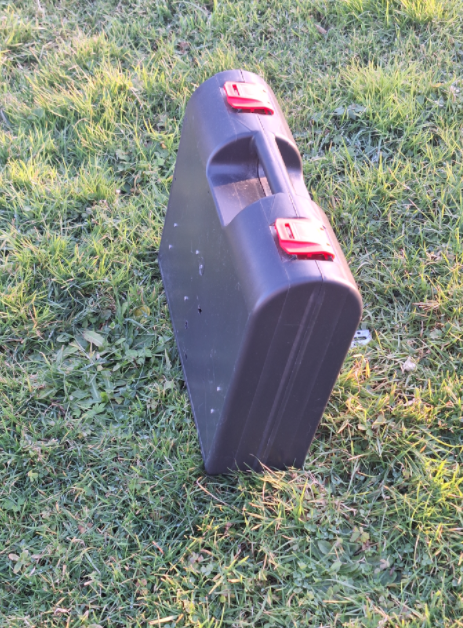
\includegraphics[width=6cm,keepaspectratio, ]{../sci/img/Pasted image 20250123184355.png}
\caption{La valise}
\label{fig:hw1}
\end{figure}


\begin{figure} [H]\centering
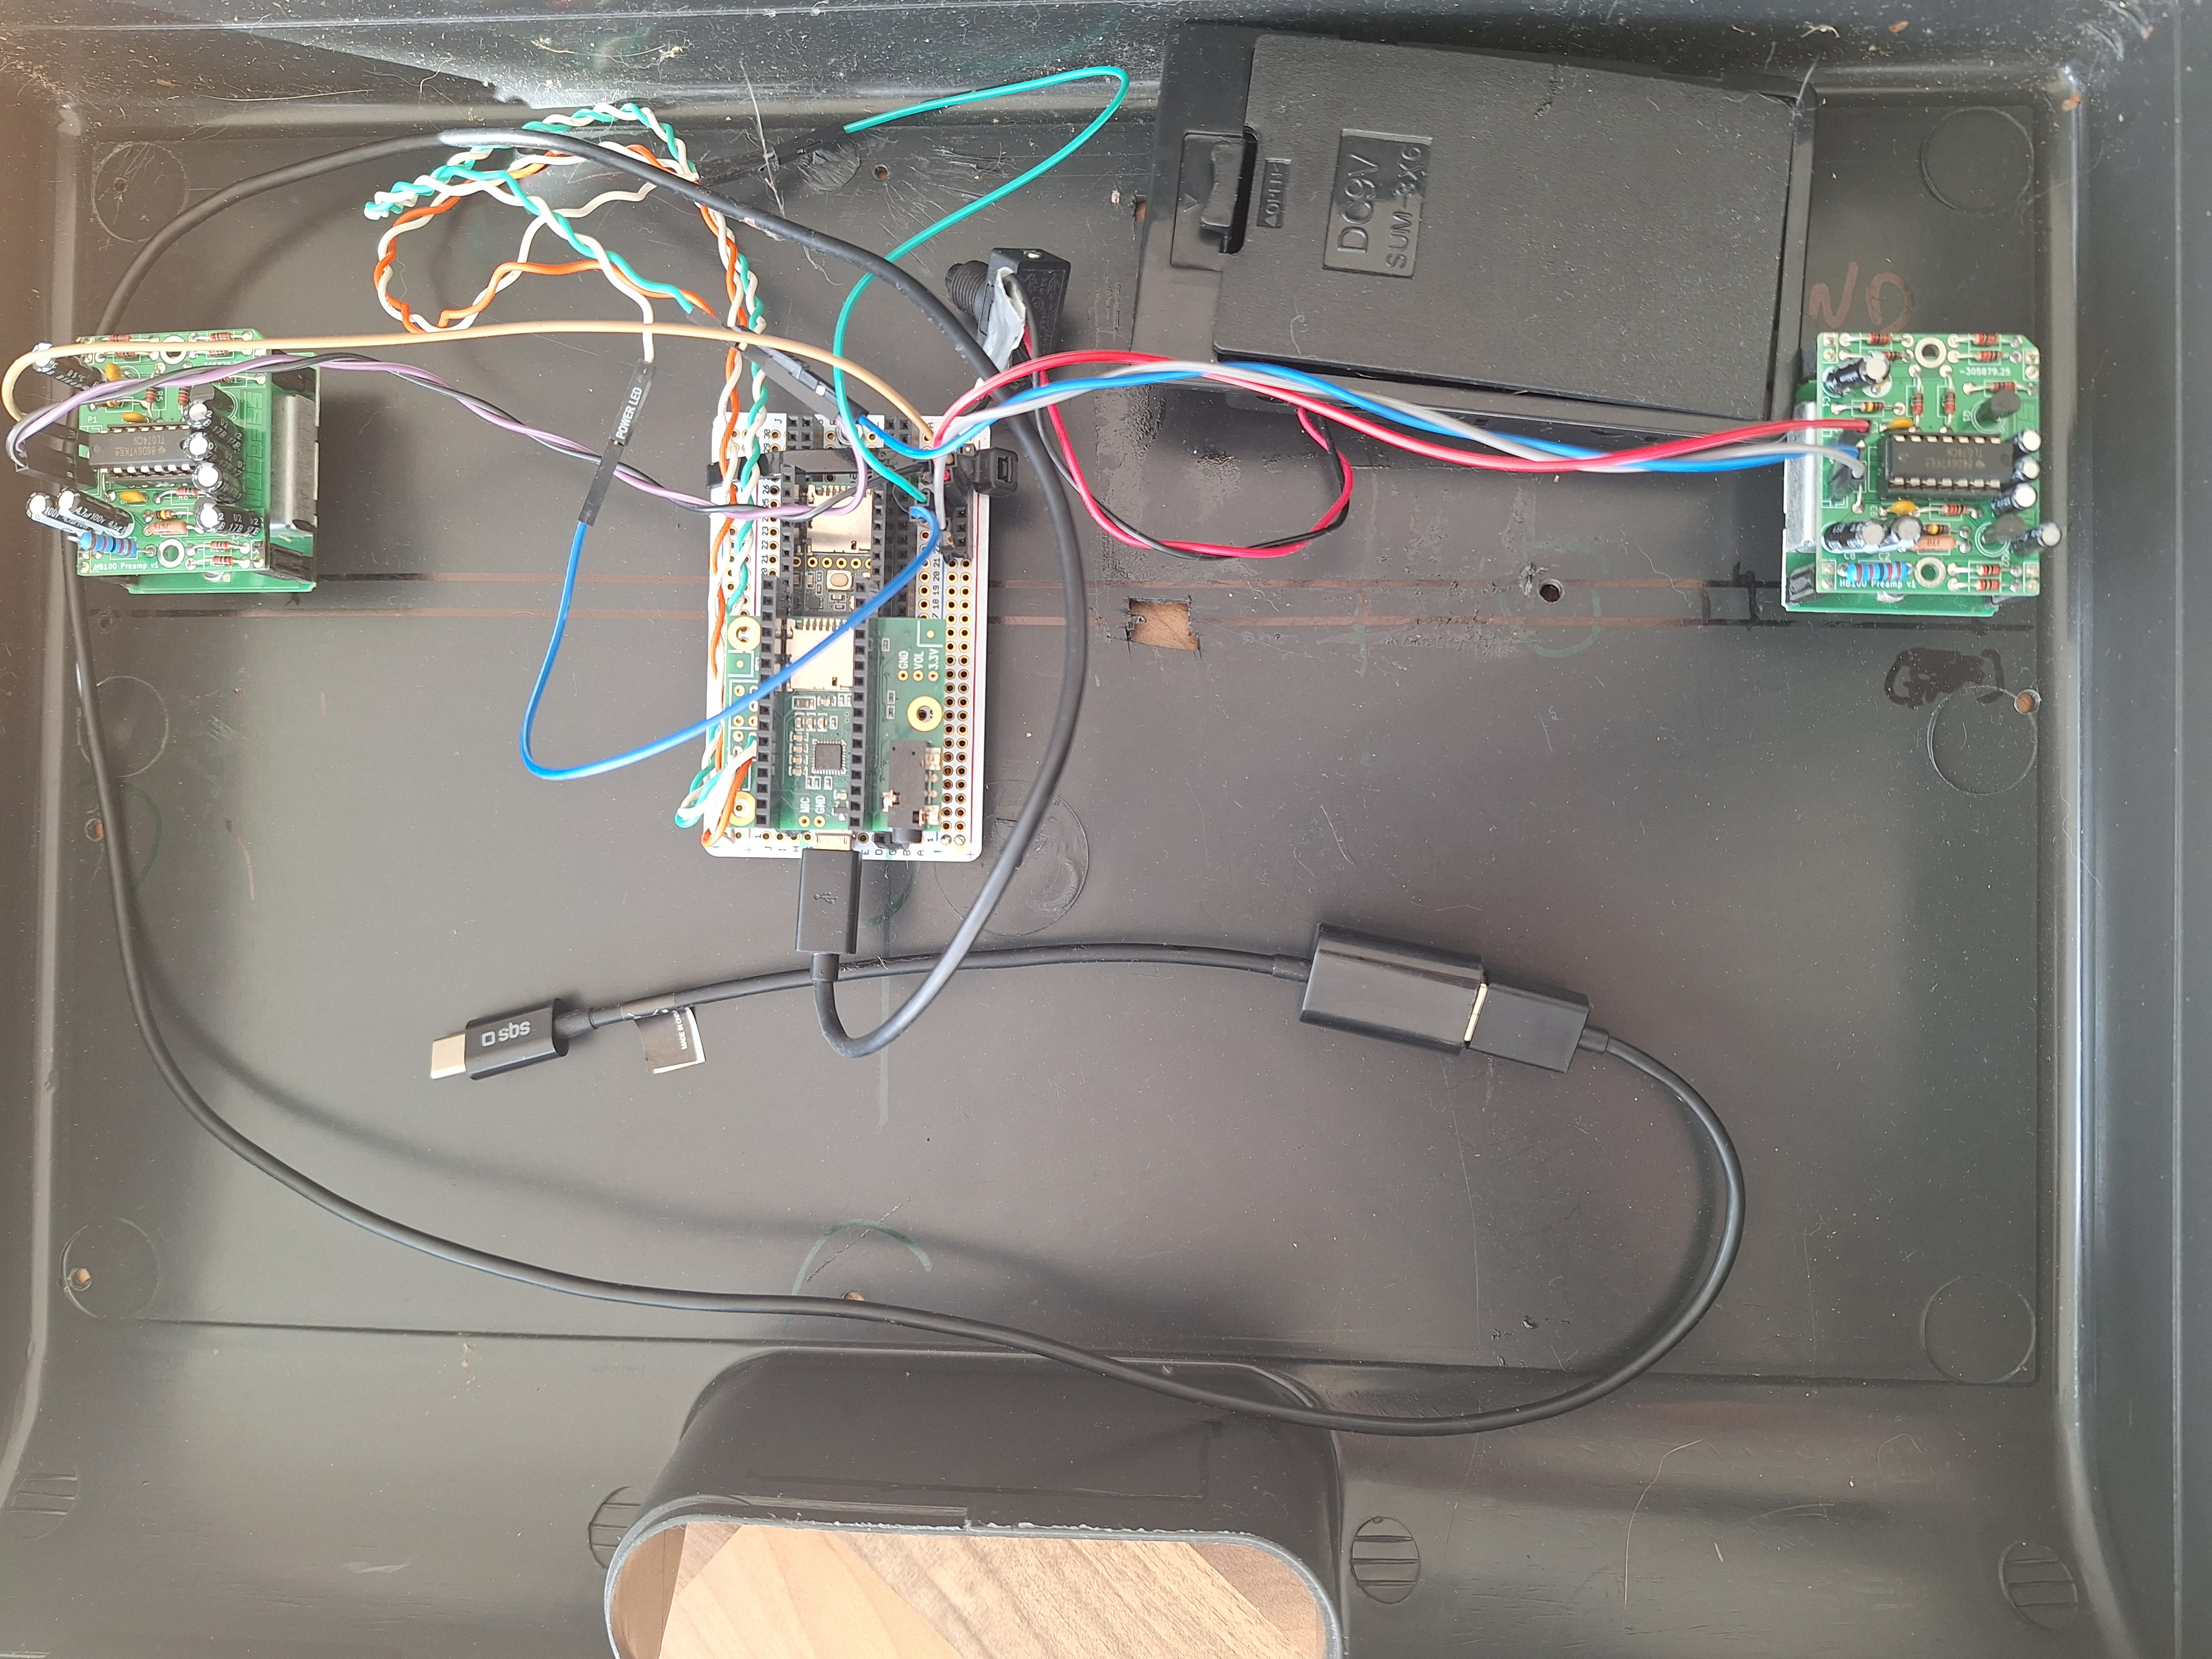
\includegraphics[width=8cm,keepaspectratio, ]{../sci/img/20250123_132304.jpg}

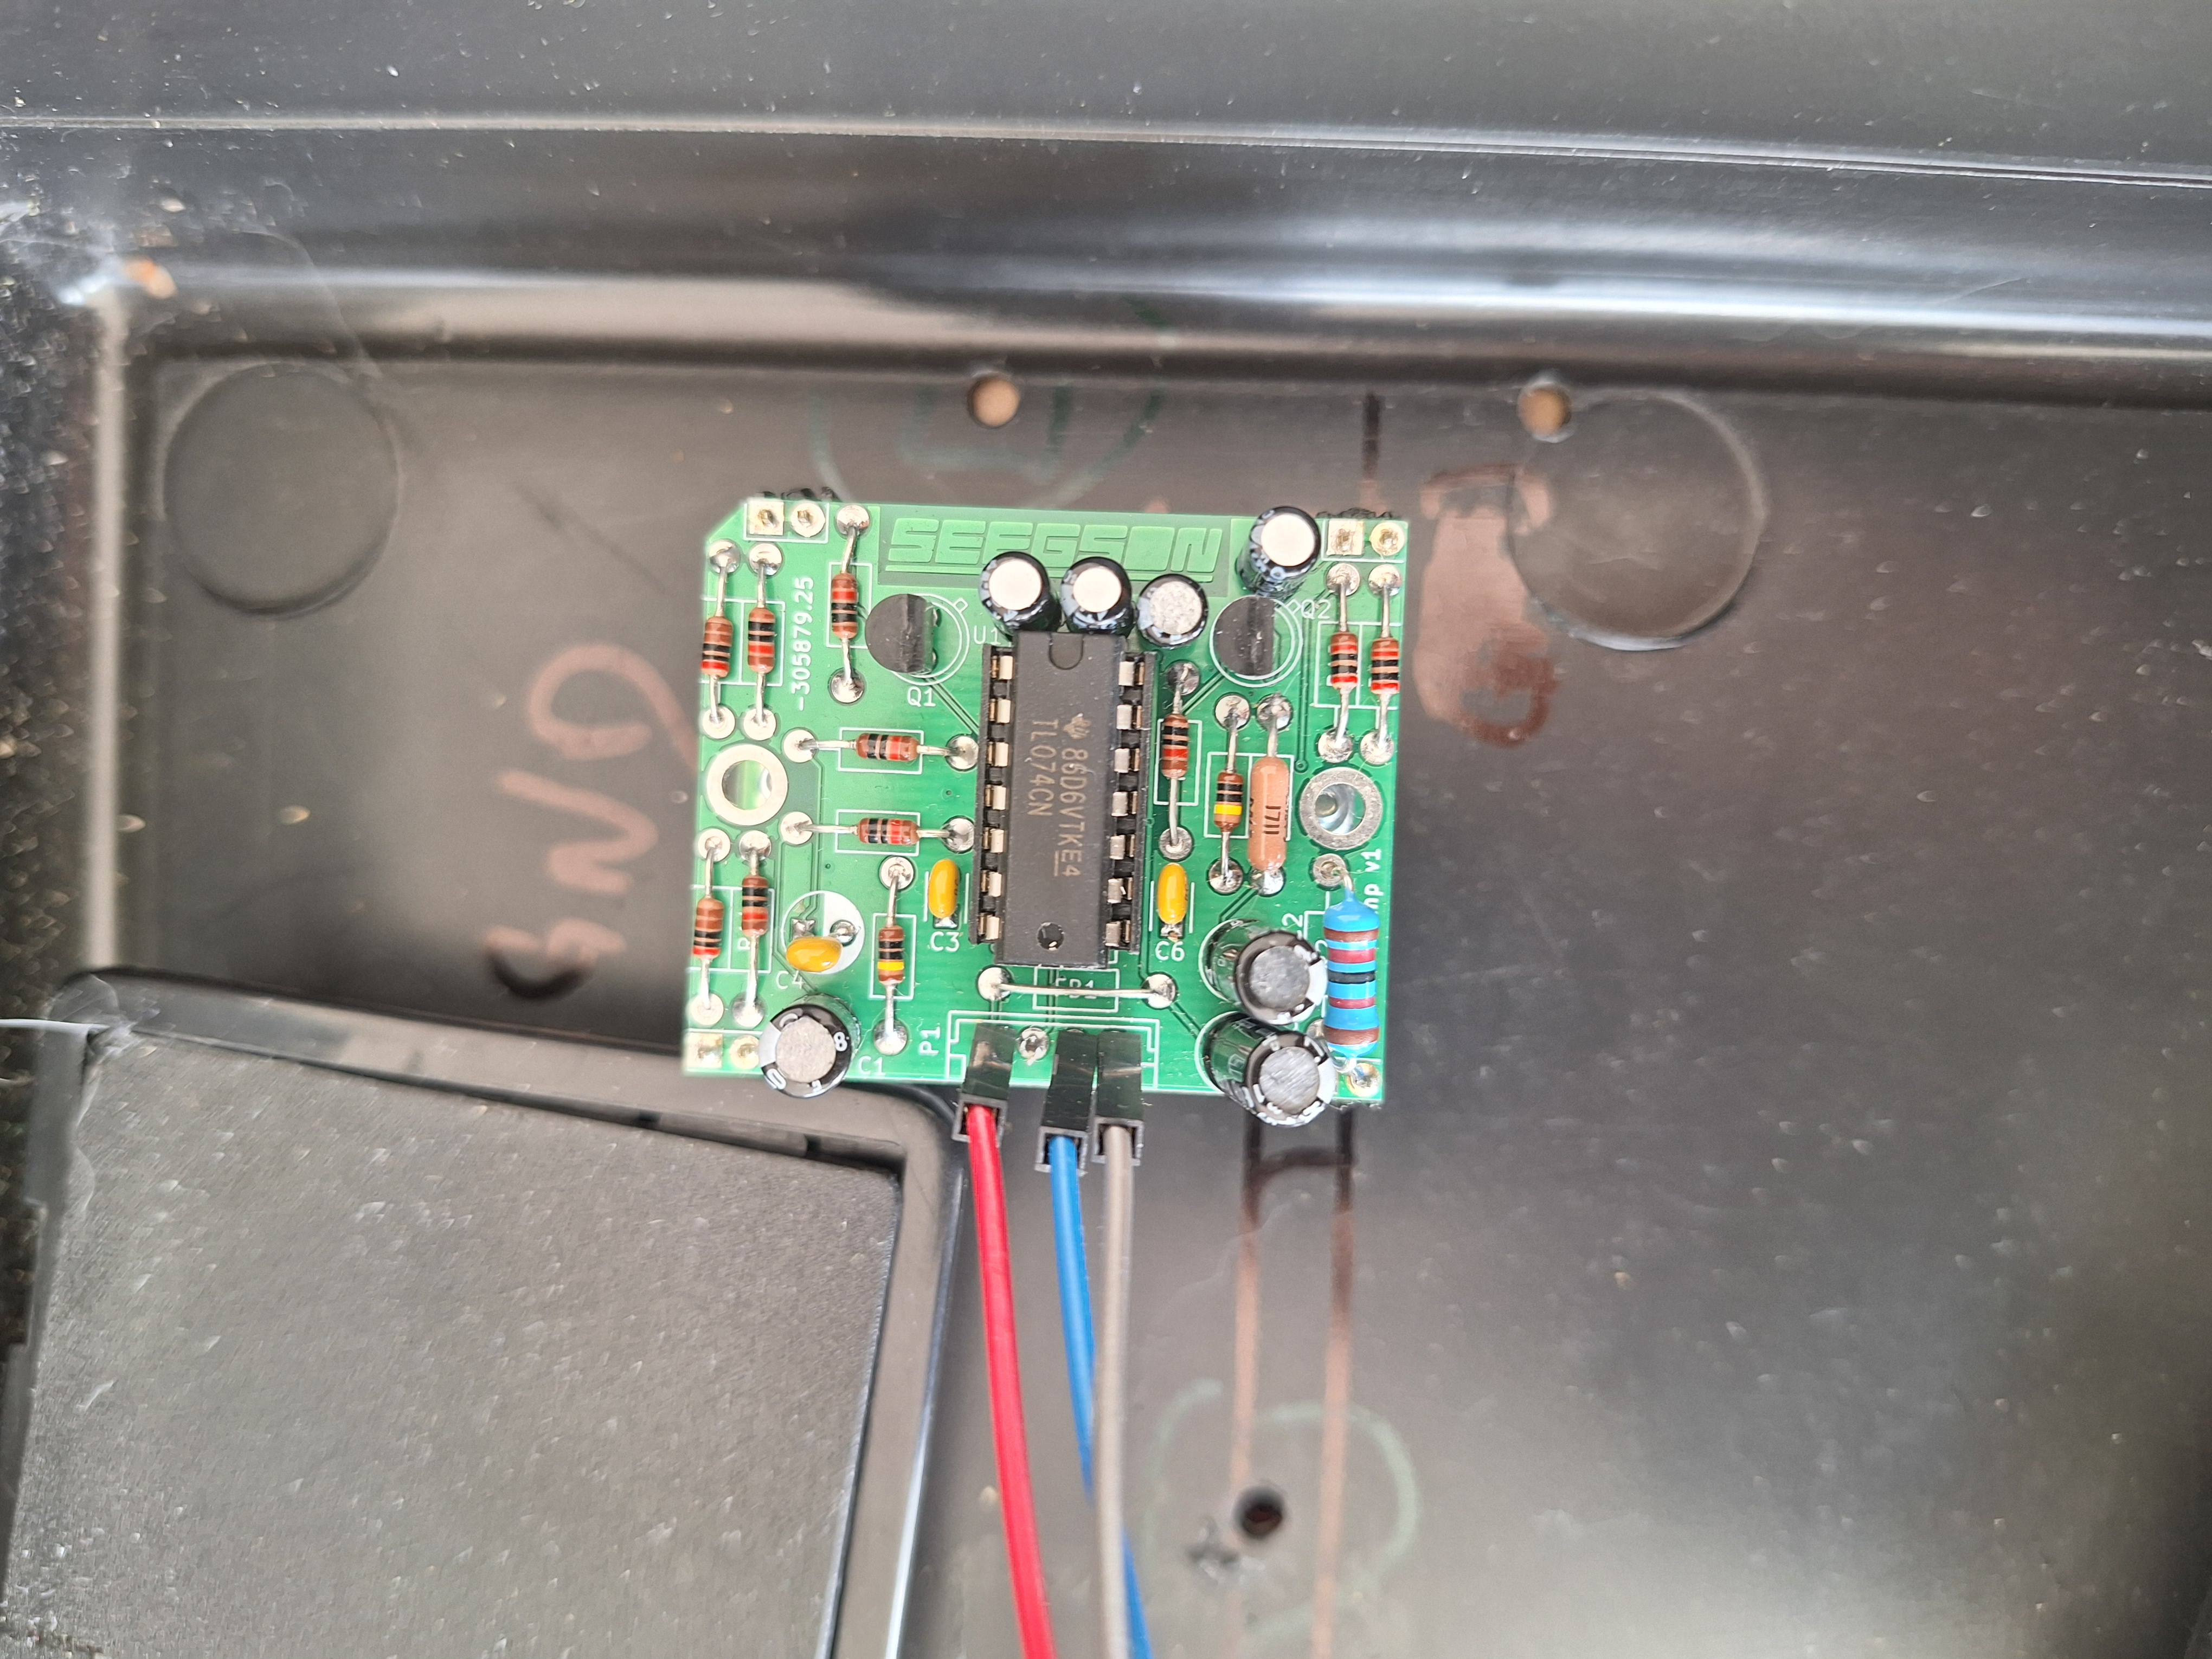
\includegraphics[width=4cm,keepaspectratio, ]{../sci/img/20250123_132310.jpg}
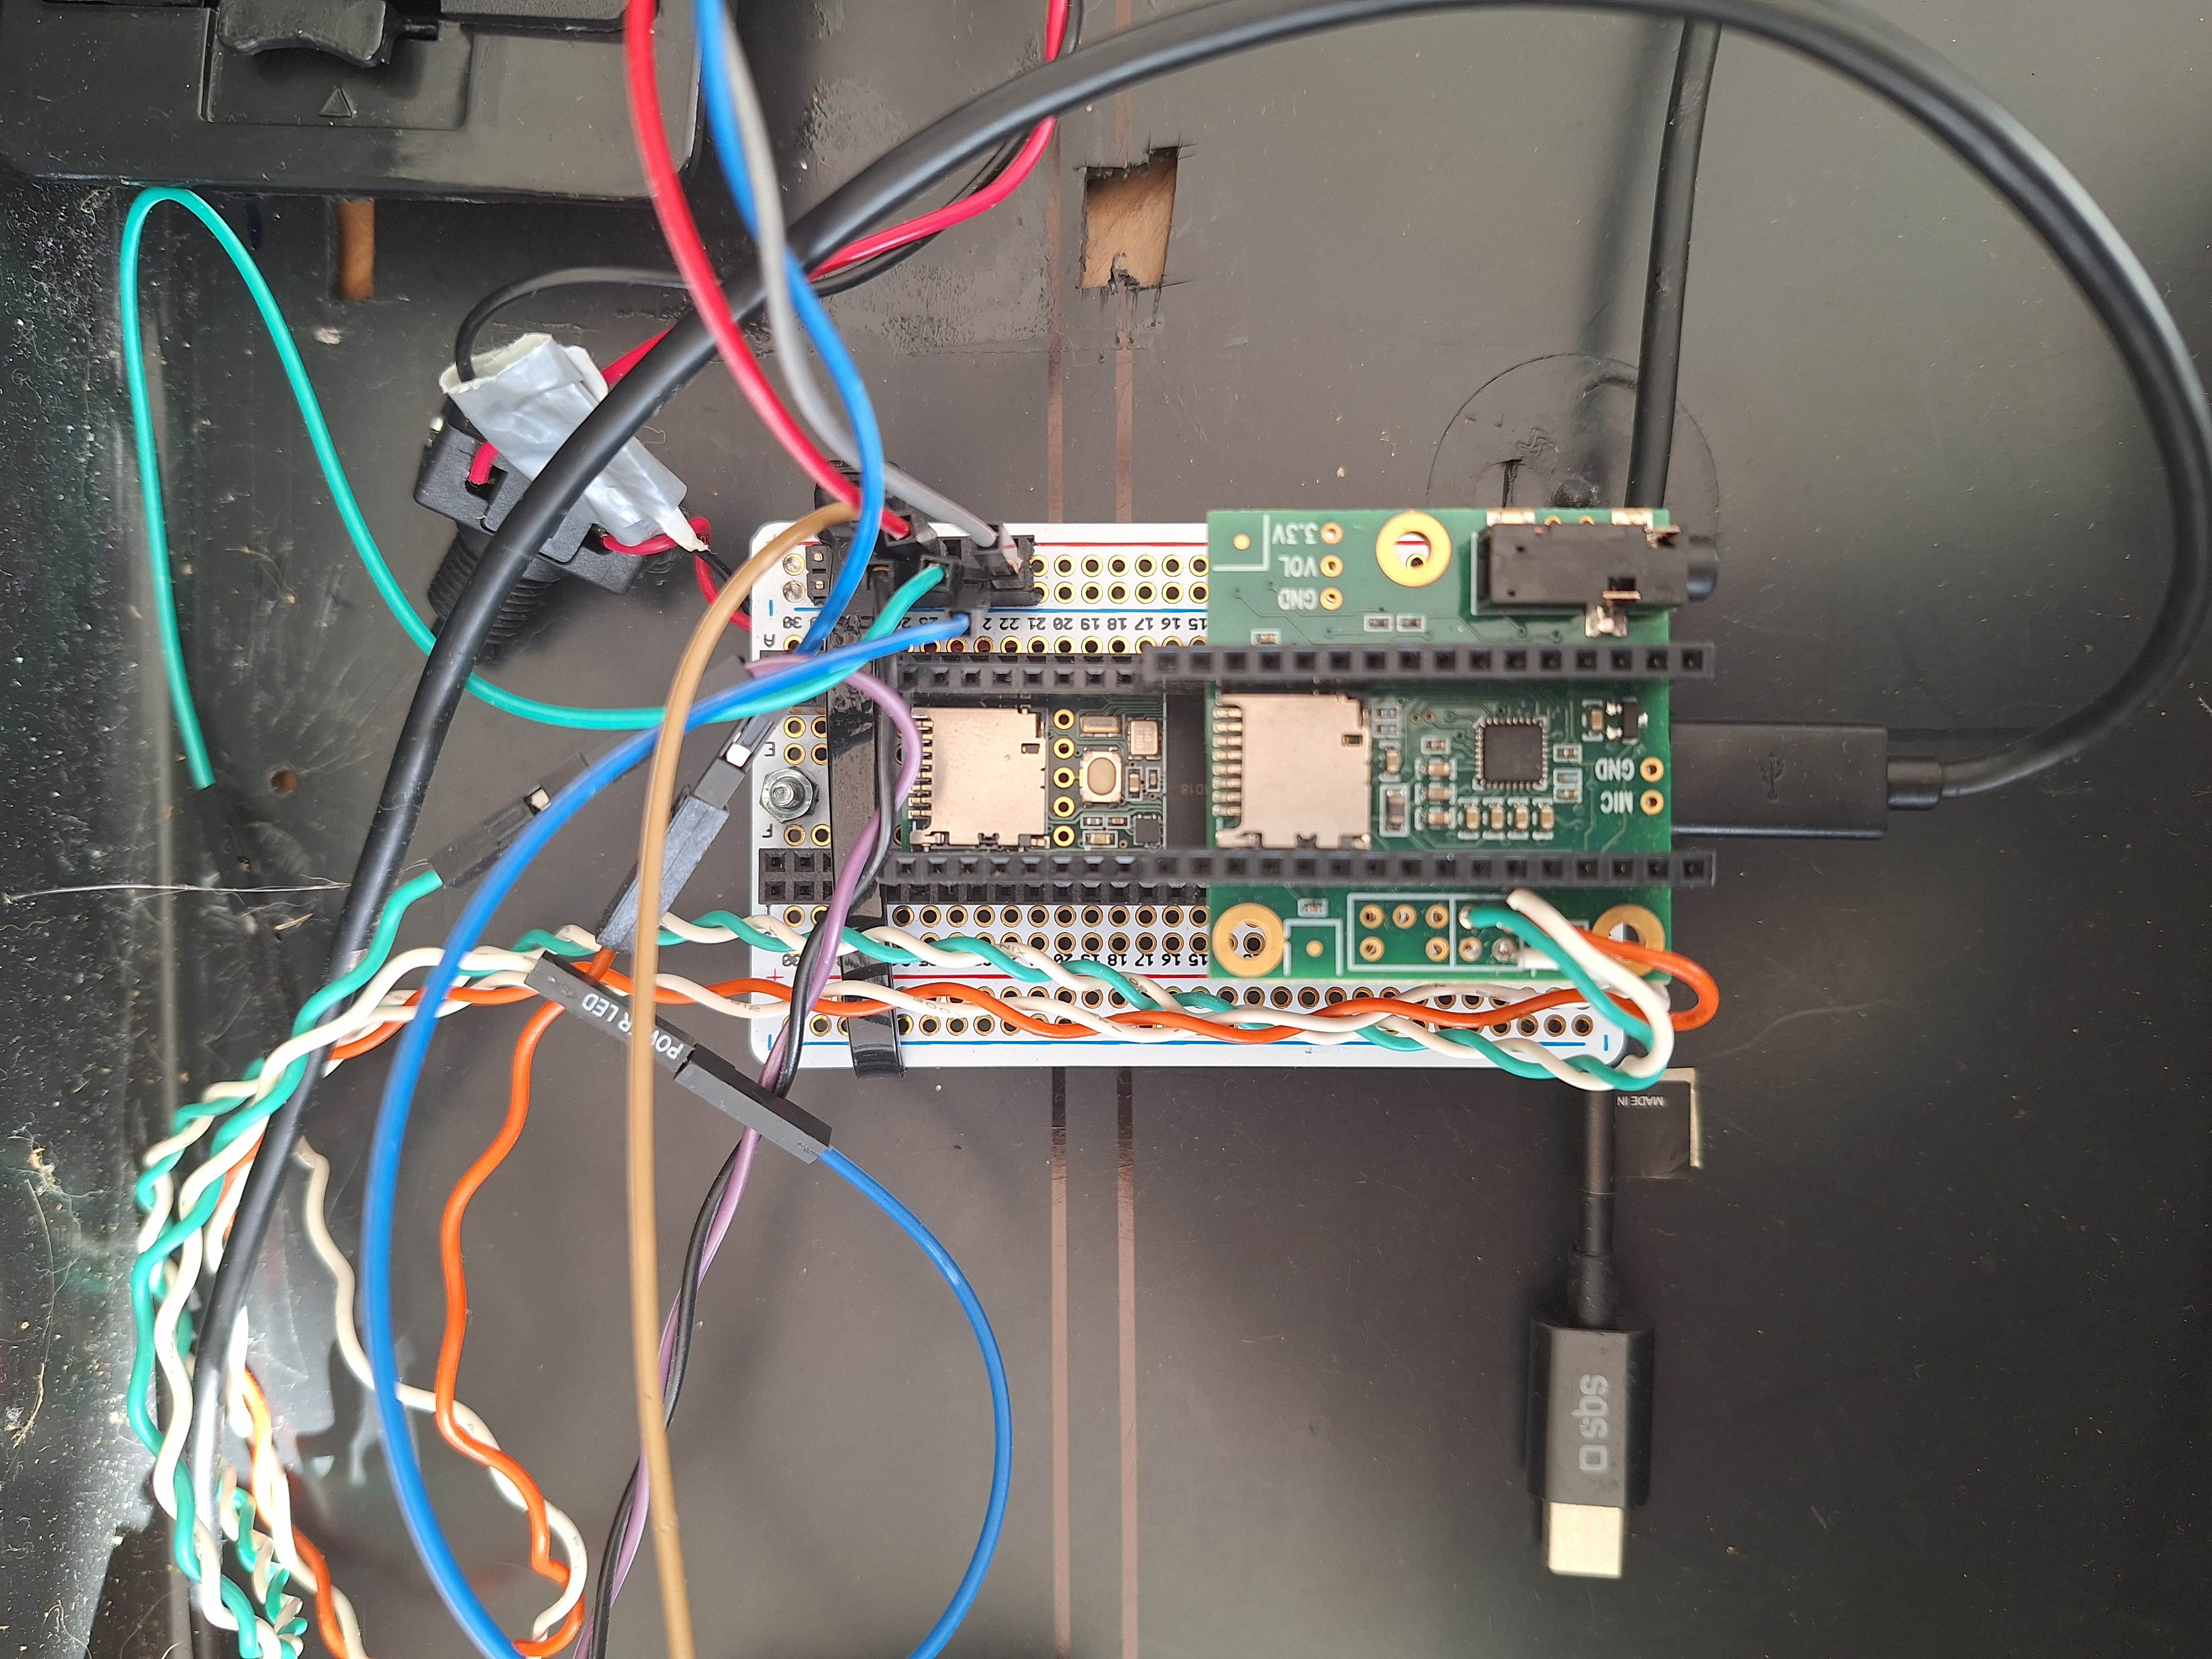
\includegraphics[width=4cm,keepaspectratio, ]{../sci/img/20250123_132345.jpg}
\caption{Intérieur avec Arduino, radar, amplificateur, cartes audio}
\label{fig:hw2}
\end{figure}


\begin{figure} [H]\centering
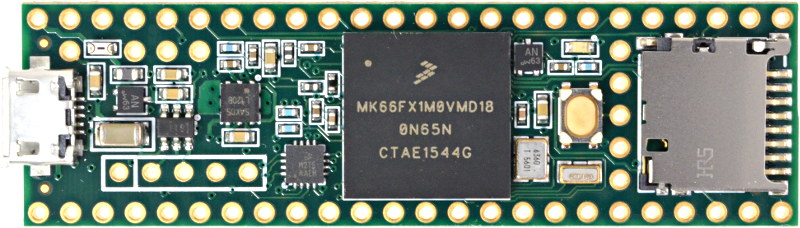
\includegraphics[width=8cm,keepaspectratio, ]{../sci/img/IMG_2427.jpg}
\caption{Tiny Arduino}
\label{fig:hw5}
\end{figure}


\begin{figure} [H]\centering
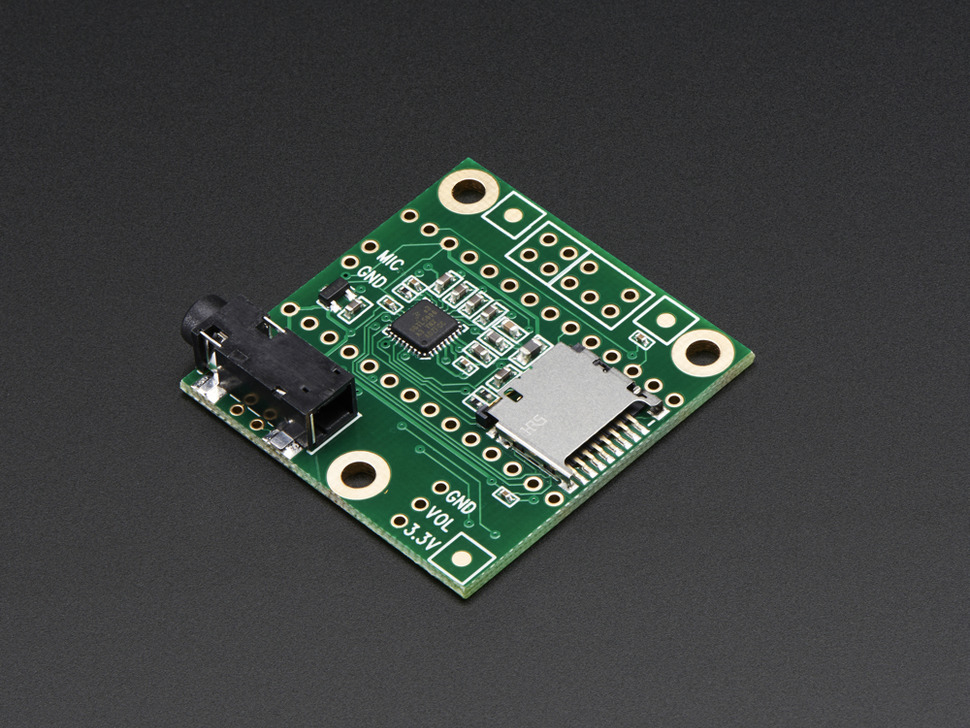
\includegraphics[width=5cm,keepaspectratio, ]{../sci/img/IMG_2428.jpeg}
\caption{Carte audio}
\label{fig:hw6}
\end{figure}

\begin{figure} [H]\centering
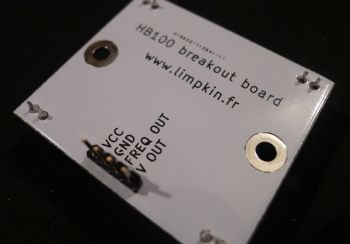
\includegraphics[width=5cm,keepaspectratio, ]{../sci/img/PCB_Back_s.jpg}
\caption{Carte amplificateur audio}
\label{fig:hw8}
\end{figure}

\begin{figure} [H]\centering
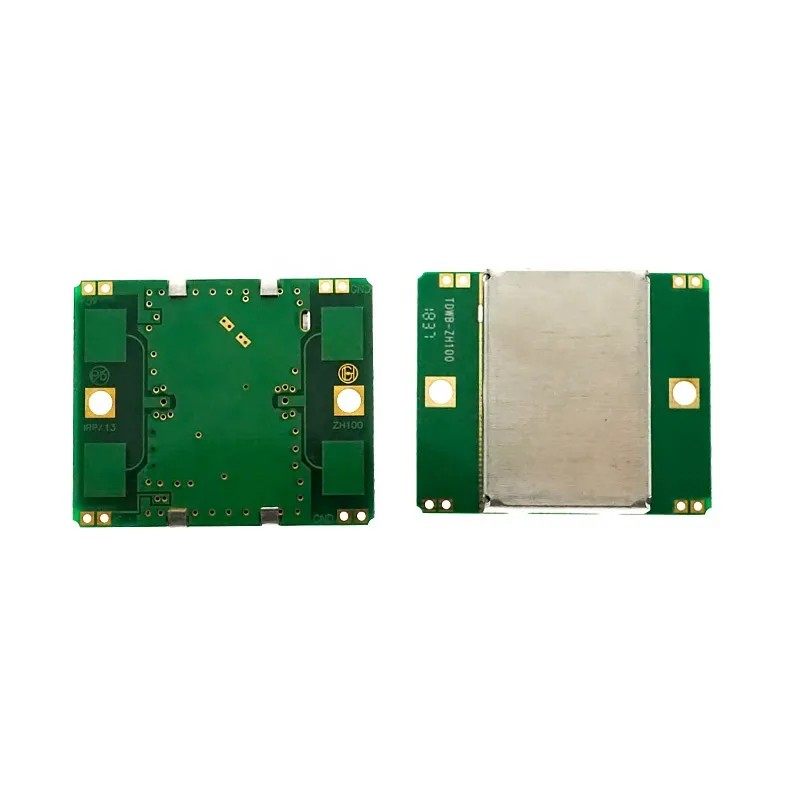
\includegraphics[width=8cm,keepaspectratio, ]{../sci/img/IMG_2429.png}
\caption{Carte radar}
\label{fig:hw7}
\end{figure}




\chapter{Analyse des données}

\section{Captures radar filtrées}

\begin{figure} [H]\centering
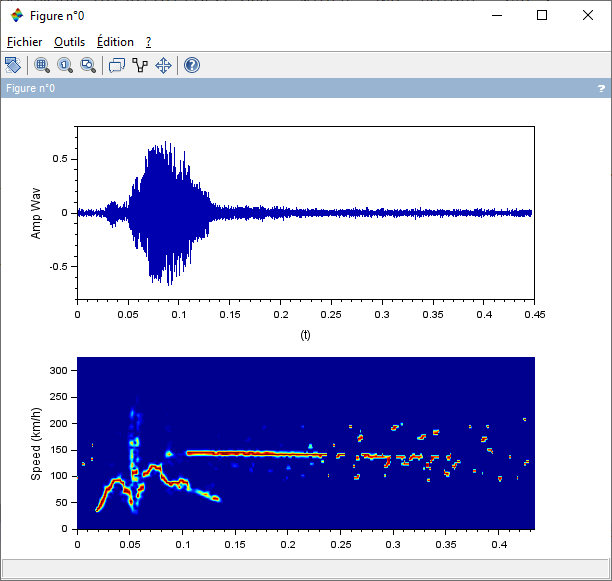
\includegraphics[width=8cm,keepaspectratio, ]{../sci/img/Pasted image 20250122083320.png}
\caption{Captures WAV radar et leur écho}
\label{fig:wavradarcapture}
\end{figure}


\subsection{Filtrage}
\begin{figure} [H]\centering
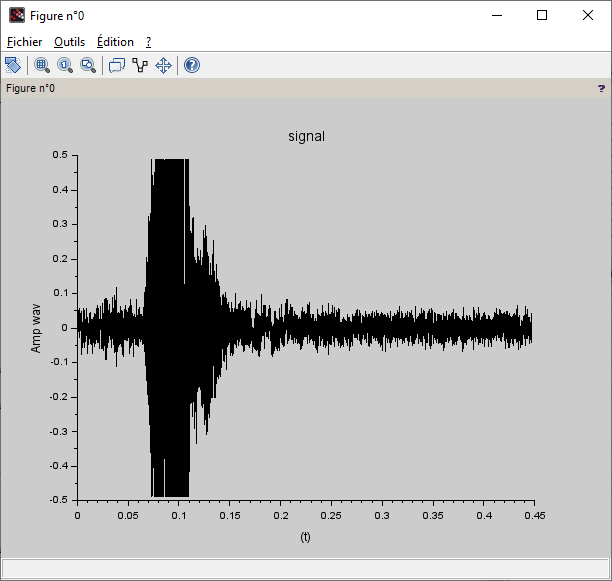
\includegraphics[width=8cm,keepaspectratio, ]{../sci/img/Pasted image 20250122082849.png}
\caption{WAV brut capturé}
\label{fig:rawcapture}
\end{figure}

\begin{figure} [H]\centering
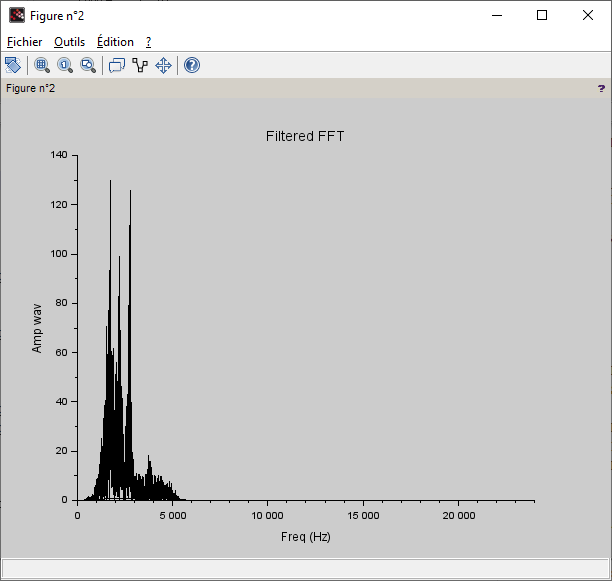
\includegraphics[width=8cm,keepaspectratio, ]{../sci/img/Pasted image 20250122082913.png}
\caption{FFT du brut filtré}
\label{fig:rawfft}
\end{figure}

\subsection{Résultat final}
\begin{figure} [H]\centering
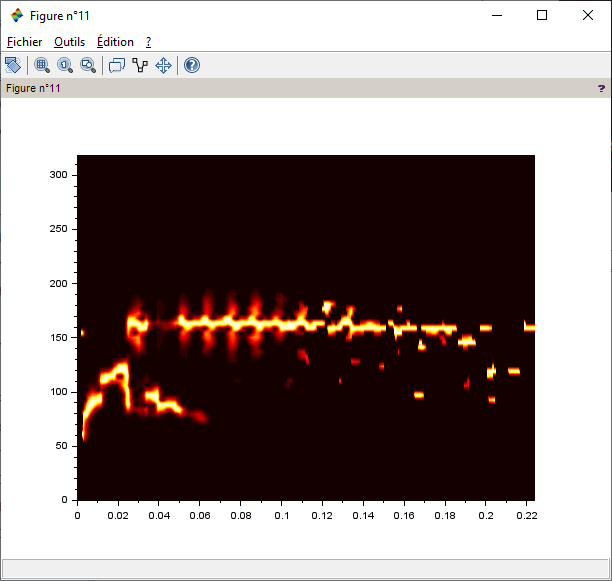
\includegraphics[width=8cm,keepaspectratio, ]{../sci/img/Pasted image 20250120172502.png}
\caption{Résultats de mon algorithme de densité de puissance pour identifier vitesse et backspin}
\label{fig:radarcapture}
\end{figure}

\begin{figure} [H]\centering
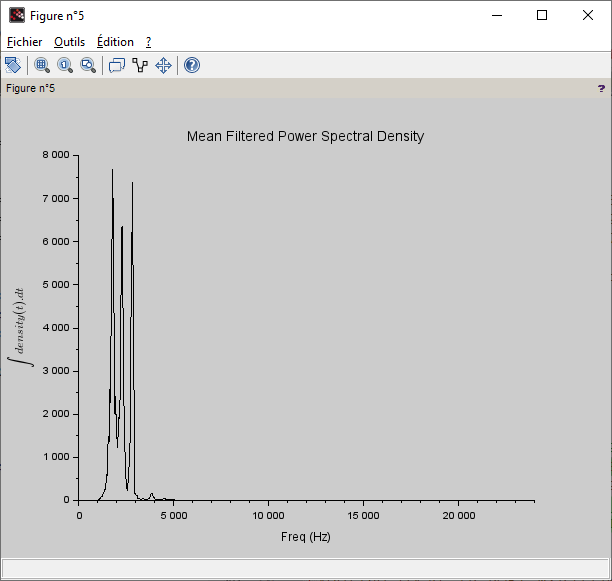
\includegraphics[width=8cm,keepaspectratio, ]{../sci/img/Pasted image 20250122082958.png}
\caption{Résultats de la densité spectrale de puissance filtrée en moyenne et normalisée}
\label{fig:filtered power density results}
\end{figure}

\begin{figure} [H]\centering
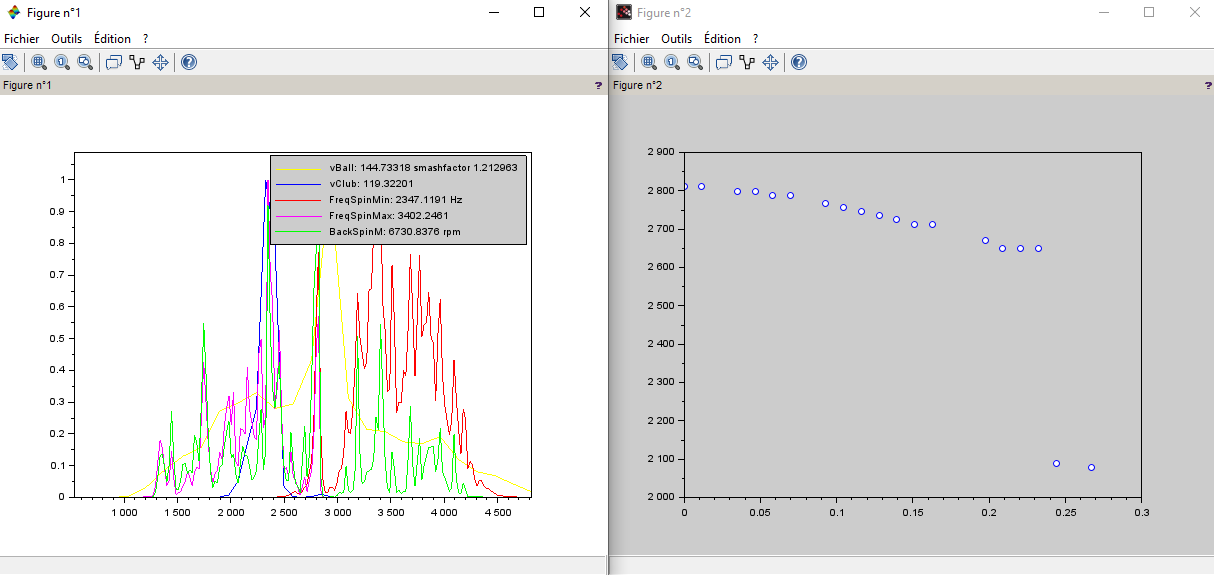
\includegraphics[width=12cm,keepaspectratio, ]{../sci/img/Pasted image 20250122083851.png}
\caption{Résultats du filtrage de la densité et de l'identification des caractéristiques}
\label{fig:identifycarac}
\end{figure}

\begin{figure} [H]\centering
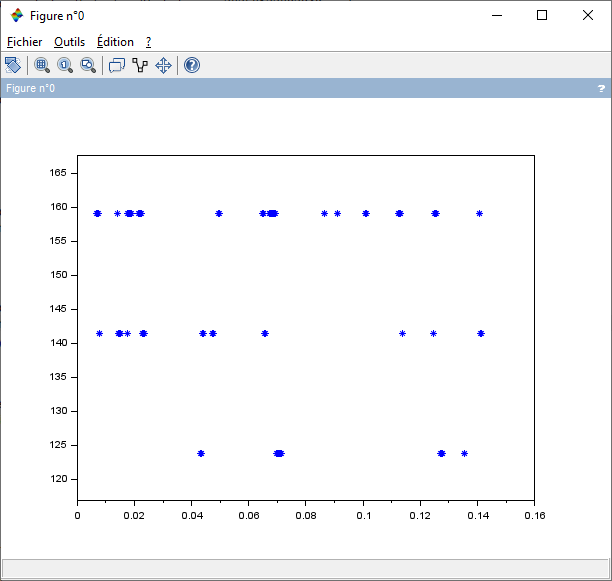
\includegraphics[width=8cm,keepaspectratio, ]{../sci/img/Pasted image 20250217094457.png}
\caption{Échos de vitesse et de backspin}
\label{fig:identifycarac}
\end{figure}


\chapter{Pipe de traitement du signal radar Doppler : de Scilab à Python}
\label{chap:radarpipe}

Ce chapitre documente la chaîne complète de traitement du signal permettant d'extraire la vitesse de la balle, le spin total et l'azimut de départ à partir des deux radars Doppler 10,525~GHz (acquisition audio à $F_s=44100$~Hz, un canal par radar), les corrections apportées au code Scilab historique (\texttt{sci/FFT\_Mat.sce}, commit \texttt{73ef2d8}), et le port Python (\texttt{sci/pipe\_validation.py}) utilisé pour la validation aveugle sur les 9 captures F7 du 2019-02-24 plus 2 signaux modèle générés.

\section{Géométrie des deux radars et observables Doppler}

Chaque radar ne mesure que la projection de la vitesse de la balle sur sa ligne de visée :
\begin{equation}
f_i = \frac{2}{\lambda}\,\vb V\cdot\vb u_i = K_V\,V_{r,i}, \qquad K_V \approx 19.49\ \text{Hz/(km/h)}, \quad \lambda = c/f_0 \approx 0.02848\ \text{m}
\end{equation}

Avec les radars en $R_1=(0,-b/2)$ et $R_2=(0,+b/2)$ dans le plan horizontal (axe $x$ = direction nominale du tir, $z$ = latéral, $b=0{,}30$~m), balle en $P=(x,z)$, $L_1\approx L_2\approx L$ :

\begin{align}
f_1 &= K\,\frac{V_x x + V_z(z+b/2)}{L}, \qquad f_2 = K\,\frac{V_x x + V_z(z-b/2)}{L}
\end{align}

En sommant, les termes en $\pm b/2$ s'annulent (mode commun) ; en soustrayant, ce sont les termes longitudinaux qui s'annulent (mode différentiel) :

\begin{align}
f_C &= \frac{f_1+f_2}{2} \approx K\,V_x \quad \text{« à quelle vitesse elle avance »} \\
f_\Delta &= \frac{f_1-f_2}{2} = K\,\frac{V_z\, b}{2L} \quad \text{« à quelle vitesse elle dérive latéralement, vue à travers la parallaxe } b/L\text{ »}
\end{align}

Le rapport redonne la pente du vecteur vitesse, c'est-à-dire la tangente de l'angle de départ horizontal $\alpha$ (angle entre $\vb V$ et l'axe $x$ dans le plan $x$--$z$) :

\begin{equation}
\boxed{\tan\alpha = \frac{V_z}{V_x} = \frac{2L}{b}\,\frac{f_\Delta}{f_C}
\quad\Longrightarrow\quad
\alpha(t) = \arctan\!\left[\frac{2L(t)}{b}\,\frac{f_\Delta(t)}{f_C(t)}\right], \qquad
L(t) = L_0 + \int_{t_0}^{t} V_x(\tau)\,d\tau }
\end{equation}

\begin{figure}[H]\centering
\begin{tikzpicture}[scale=1.3, >=Stealth, font=\small]
  \draw[->] (0,0) -- (6.4,0) node[right] {$x$ (direction du tir)};
  \draw[->] (3,-1.6) -- (3,2.4) node[above] {$z$ (latéral)};
  \fill (3,-1) circle (2pt) node[below] {R1};
  \fill (3,1)  circle (2pt) node[above] {R2};
  \draw[<->] (3.18,-1) -- (3.18,1) node[right, midway] {$b$};
  \fill (5.6,0.7) circle (3pt) node[above right] {P};
  \draw[dashed] (3,-1) -- (5.6,0.7);
  \draw[dashed] (3,1)  -- (5.6,0.7);
  \draw[->, very thick, red] (5.6,0.7) -- (6.5,1.25) node[right] {$\vb V$};
  \draw (6.2,0.7) arc[start angle=0, end angle=31, radius=0.6];
  \node at (6.35,0.88) {$\alpha$};
  \draw[<->] (3,-0.25) -- (5.6,-0.25) node[midway, below] {$L$};
  \node[red] at (5.2,1.45) {$V_x = V\cos\alpha$};
  \node[red, rotate=90] at (6.75,1.0) {$V_z = V\sin\alpha$};
\end{tikzpicture}
\caption{Vue de dessus du dispositif à deux radars. $f_C$ porte $V_x$ (vitesse), $f_\Delta$ porte $V_z$ (azimut $\alpha$ dans le plan $x$--$z$). Le facteur $2L/b$ corrige la parallaxe : plus la balle est loin, plus la différence de fréquence est faible pour le même $V_z$.}
\label{fig:geom2radars}
\end{figure}

\section{STFT et suivi du ridge}

Pour chaque canal, une transformée de Fourier à court terme donne le spectrogramme $P_i(k,m)=|X_i(k,m)|^2$ :
\begin{itemize}
  \item Scilab \texttt{animDensite} (\texttt{FFT\_Mat.sce}) : fenêtre de Hann 512, pas 16, seuillage en dB par trame, normalisé par le max de la trame ;
  \item Python \texttt{spectrogram} (\texttt{pipe\_validation.py}) : fenêtre de Hann $N=2048$ (46~ms), pas 1024 (recouvrement 50\%), interpolation parabolique sous-bin du pic.
\end{itemize}

La fréquence ridge de la trame $m$ est le bin du pic affiné par une parabole :
\begin{equation}
k^* = \arg\max_k P_m(k), \qquad
\delta = \frac{0.5\,(P_{k^*-1}-P_{k^*+1})}{P_{k^*-1}-2P_{k^*}+P_{k^*+1}}, \qquad
f_{ridge}(m) = (k^*+\delta)\,\frac{F_s}{N}
\end{equation}

L'instant d'impact est la trame la plus énergétique (le club métallique donne un écho fort, écrêté) :
\begin{equation}
t_0 = \arg\max_m \sum_k P_m(k)
\end{equation}

\section{Vitesse : médiane du ridge post-impact vs max global}

Le max global du spectre sommé dans le temps, $\hat f_B = f_5[\arg\max_k \sum_m M_5(m,k)^2]$ (Scilab \texttt{Info}), est dominé par le fort écho du club écrêté (6,6--14,8\% des échantillons à $\pm0{,}489$), dont le spectre est large et plat. La balle produit un ridge étroit qui \emph{durée} tout le vol. D'où l'estimateur Python :
\begin{equation}
\hat V = \frac{1}{19.49}\,\operatorname*{median}_{m\in[t_0,\,t_0+50\,\text{ms}]} f_{ridge}(m)
\end{equation}
Chaque trame vote pour une fréquence, sans pondération : la médiane tolère jusqu'à 50\% de trames aberrantes (résidu du club, faux lobes), tandis que la somme pondérée par l'énergie laisse une seule trame fausse mais forte tirer le résultat. Mesuré sur les 11 CSV : MAE 5,7\% radiale, 1,9\% après correction géométrique $\cos 20^\circ$. Sur microcontrôleur (Arduino), la détection d'impact est en $O(1)$ par trame et un max sur la fenêtre post-impact suffit quand $t_0$ est fiable ; la médiane est la marge de sécurité quand il ne l'est pas.

\section{Spin : périodicité du patch vs excursion spectrale}

La balle est partiellement recouverte de ruban aluminium (un diffuseur dominant, « le patch »). Deux estimateurs du spin \emph{total} existent :

\begin{enumerate}
  \item \textbf{Excursion spectrale} (Scilab \texttt{GetSwing}/\texttt{Info2}) : la vitesse du point de surface est $v_t = r\omega$, donc l'étalement Doppler est
  \begin{equation}
  \Delta f_{spin} = \frac{f_+ - f_-}{2} = \frac{2r\omega}{\lambda}, \qquad
  SpinTotal_{RPM} = \frac{\Delta f_{spin}}{K_S}, \quad K_S \approx 0.1567\ \text{Hz/RPM}
  \end{equation}
  Cela utilise les deux \emph{bords extrêmes} du spectre micro-Doppler -- les points les plus faibles, donc les plus noyés dans le bruit et l'écrêtage ADC. MAE mesurée : 41,4\% (\texttt{GetSwing}) à 51--68\% (variantes).

  \item \textbf{Périodicité du patch} (Python) : le patch produit un « flash » radar par tour, quelle que soit l'inclinaison $\beta$ de l'axe de spin, donc l'enveloppe de Hilbert du signal post-impact contient une raie à
  \begin{equation}
  f_{rot} = \frac{SpinTotal}{60} \quad\Longrightarrow\quad \boxed{SpinTotal_{period} = 60\,f_{rot}}
  \end{equation}
  $f_{rot}$ est le pic du spectre d'enveloppe au meilleur score d'harmoniques $\sum_q P(k_q)$ pour $f_q \approx k f_{rot}$ (évite les sous-harmoniques et le cas dégénéré à 2 flashs par tour quand l'axe de spin est aligné avec la ligne de visée). MAE mesurée : \textbf{19,9\%} sur les 9 vrais coups, et \textbf{$-0{,}1$\%} (3996 vs 4000~tr/min) sur le signal modèle propre.
\end{enumerate}

Les deux estimateurs mesurent le spin \emph{total} $\omega = \sqrt{\omega_{back}^2+\omega_{side}^2}$, pas le backspin : la fréquence du flash vaut $\omega/2\pi$ quel que soit $\beta$, et l'excursion vaut $2r\omega/\lambda$. Séparer BackSpin/SideSpin exige $\beta$, identifié ailleurs (courbure de $\alpha(t)$, ou le \texttt{SpinAxis} de \texttt{GetSwing} : $\beta \approx \operatorname{asin}[Spin_3/\sqrt{((Spin_1+Spin_2)/2)^2+Spin_3^2}]$ — qualitatif seulement : MAE $\approx 15$--$18^\circ$).

\begin{figure}[H]\centering
\begin{tikzpicture}[scale=1.2, >=Stealth, font=\small]
  \draw[thick] (0,0) circle (1.4);
  \fill[gray!60] (0,0) -- (30:1.4) arc[start angle=30, end angle=80, radius=1.4] -- cycle;
  \node at (55:1.05) {patch};
  \draw[->, very thick] (0,0) -- (0.7,1.9) node[above] {$\vb\omega$ (axe incliné de $\beta$)};
  \draw[dashed, ->] (-3.2,0.6) -- (-1.5,0.25) node[left] {radar};
  \draw[->] (0,0) -- (1.4,0) node[right] {$r$};
  \node at (0,-1.9) {flash 1 fois/tour : $f_{rot}=\omega/2\pi$};
  \node at (0,-2.4) {excursion : $\Delta f = 2r\omega/\lambda$};
\end{tikzpicture}
\caption{Le patch aluminium comme diffuseur dominant unique. La périodicité du flash comme l'excursion spectrale mesurent le spin \emph{total} $\omega$ ; aucune des deux ne sépare backspin et sidespin.}
\label{fig:patch}
\end{figure}

\section{Appariement stéréo des deux ridges}

Suivre indépendamment le max FFT de chaque radar peut choisir deux lobes micro-Doppler différents et produire un faux azimut (erreurs $>20^\circ$ observées). Le tracker Python les apparie : connaissant $f_1$ (ridge de R1), $f_2$ est cherché dans le spectre de R2 à $\pm 300$~Hz de $f_1$, avec la contrainte de cohérence $|f_1-f_2| \lesssim 30$~Hz (géométrie, $b=0{,}30$~m). Puis $\alpha(t)$ découle de l'équation ci-dessus, avec
\begin{equation}
\alpha_0 = \operatorname*{median}_{t\in[t_0,t_0+50\,\text{ms}]}\alpha(t), \qquad
\Delta\alpha_{BF} = \operatorname*{median}_{W_F}(\alpha) - \operatorname*{median}_{W_0}(\alpha)
\end{equation}
Mesuré : $\alpha_0$ résolu 9/9 ($-3{,}1^\circ$ à $-0{,}2^\circ$) ; signe de $\Delta\alpha$ vs sidespin de référence 0/9 car les fichiers de référence n'encodent que $|$sidespin$|$ (le dataset signé gauche/droite est la prochaine priorité).

\section{Contrôles qualité (« non identifiable » est une sortie valide)}
\begin{itemize}
  \item symétrie des bords micro-Doppler : $|(f_C-f_-)-(f_+-f_C)| < \eta\,\Delta f_{spin}$, $\eta=0{,}2$ ;
  \item cohérence inter-radars : $|Spin_1-Spin_2|/\mathrm{moyenne} < 20\%$ ;
  \item concordance excursion/périodicité $<20\%$ pour fusionner les deux estimateurs de spin, sinon périodicité seule ;
  \item divergence de vitesse inter-radars $>15\%$ $\Rightarrow$ rejet du canal au faux lobe ;
  \item objectifs de validation : MAE$_V<2$~km/h, MAE$_{spin}<500$~tr/min (8\%), MAE$_{\alpha_0}<1^\circ$, $>90\%$ de signes de courbure corrects, MAE$_\beta<7^\circ$ puis $3$--$5^\circ$.
\end{itemize}

\section{Scilab $\rightarrow$ Python : corrections et résultats de validation}

Corrections commitées dans \texttt{sci/FFT\_Mat.sce} (commit \texttt{73ef2d8}, mergées dans \texttt{main}) :
\begin{itemize}
  \item \texttt{deltaF} : ajout du facteur $3{,}6$ manquant (km/h $\to$ m/s) et harmonisation de $r=0{,}04267/2$, désormais cohérent avec \texttt{Freq2RpmSpin} ;
  \item \texttt{animDensite2/3} : garder la \emph{moitié basse} du spectre ($M1(:,1:\$/2)$) correspondant au vecteur fréquence (avant : \texttt{\$/2:\$-1}, moitié haute, mapping cassé) ; seuillage mis à 0 au lieu de $-1000$ (qui écrasait le pic après normalisation) ;
  \item \texttt{Enveloppe} : démodulation I/Q à la porteuse centrale $f_c=(f_b+f_h)/2$ au lieu de $\cos(t\cdot F_s)=\cos(n)$ (démodulation à $F_s/2\pi\approx 7$~kHz, hors bande).
\end{itemize}

Validation aveugle sur les 11 fichiers CSV (références encodées dans les noms de fichiers), port des pipes Scilab exacts (README « Simples Scilab Commands » + \texttt{testsFFT.sci} ligne 1029) vs le pipe Python :

\begin{table}[H]\centering
\caption{Résultats mesurés, 11 CSV (9 vrais coups F7 + 2 signaux modèle).}
\label{tab:scilabvspython}
\small
\begin{tabular}{|l|c|c|c|}
\hline
Estimateur & MAE $V_{balle}$ radiale & MAE corr. $\cos20^\circ$ & MAE SpinTotal \\ \hline
Scilab \texttt{GetSwing} (port) & 5,7\% & $\approx$1,9\% & 41,4\% (excursion) \\
Variantes robustes Scilab & 5,7\% & $\approx$1,9\% & 60--68\% \\
Python \texttt{pipe\_validation.py} & \textbf{5,7\%} & \textbf{1,9\%} & \textbf{19,9\%} (périodicité) \\ \hline
\end{tabular}
\end{table}

Conclusion : la chaîne Scilab est \emph{bonne pour la vitesse et l'impact} (MAE identique au Python) et indicative pour le spin ; le pipe Python ajoute l'estimateur de spin par périodicité du patch, l'appariement stéréo pour $\alpha$, et les contrôles qualité -- les gains viennent du choix du bon observable, pas d'une mathématique plus lourde.

\section{Pipe de traitement}

\begin{figure}[H]\centering
\begin{tikzpicture}[node distance=5mm and 6mm, box/.style={draw, rounded corners, align=center, font=\footnotesize, inner sep=3pt}, >=Stealth]
  \node[box] (csv) {CSV 2 canaux R1/R2 \\ ($F_s=44100$)};
  \node[box, below=of csv] (bp) {passe-bande 1--6 kHz};
  \node[box, below=of bp] (stft) {STFT Hann 2048, hop 1024 \\ $P_m(k)=|X_m(k)|^2$};
  \node[box, below=of stft] (t0) {$t_0=\arg\max_m\sum_k P_m(k)$ (impact)};
  \node[box, below left=of t0] (ridge) {ridge $f_{ridge}(m)$ \\ parabole $\delta$};
  \node[box, below right=of t0] (pair) {appariement stéréo : $f_2$ près de $f_1$ \\ $|f_1-f_2|\le30$ Hz};
  \node[box, below=of ridge] (v) {$\hat V=\mathrm{median}_{m>t_0} f_{ridge}/19.49$};
  \node[box, below=of pair] (al) {$f_C,f_\Delta\Rightarrow\alpha(t),\alpha_0,\Delta\alpha$};
  \node[box, below left=of v, xshift=-1cm] (edge) {bords $f_\pm$ : $Spin_{edge}$, sym. $\eta$};
  \node[box, below right=of v, xshift=1cm] (per) {Hilbert 250 ms : $Spin_{period}=60f_{rot}$};
  \node[box, below=of v, yshift=-1.2cm] (agg) {fusion + contrôles qualité \\ sinon « non identifiable »};
  \draw[->] (csv) -- (bp); \draw[->] (bp) -- (stft); \draw[->] (stft) -- (t0);
  \draw[->] (t0) -- (ridge); \draw[->] (t0) -- (pair);
  \draw[->] (ridge) -- (v); \draw[->] (pair) -- (al);
  \draw[->] (stft) -| (edge); \draw[->] (stft) -| (per);
  \draw[->] (v) -- (agg); \draw[->] (edge) -| (agg); \draw[->] (per) -| (agg);
\end{tikzpicture}
\caption{Pipe de validation Python (\texttt{sci/pipe\_validation.py}). Équivalents Scilab : \texttt{animDensite} (STFT), \texttt{Info}/\texttt{GetSwing} (vitesse), \texttt{animHilbert} (enveloppe), \texttt{acos(f2/f1)} (azimut rudimentaire dans \texttt{testsFFT.sci}).}
\label{fig:pipepython}
\end{figure}

\section{Spectrogrammes : captures mesurées vs modèle théorique}

Les figures suivantes montrent les spectrogrammes mesurés des captures F7 du 2019-02-24 (R1/R2, axe vertical en km/h via $f/19.49$, ridge de la balle en cyan, impact marqué), et les captures \emph{générées} théoriques. Le signal modèle (\texttt{gen\_capture\_modele.py}) est une porteuse Doppler à laquelle s'ajoute la modulation de phase du patch $e^{-i(2r/\lambda)\sin\omega t}$, un pic de club à $t_0=100$~ms et un bruit de 28~dB. Les captures modèle sont les références de ce que le traitement \emph{devrait} obtenir sur un signal propre -- sur le coup modèle de 102~m, le pipe retrouve le spin à $-0{,}1$\%.

\begin{figure}[H]\centering
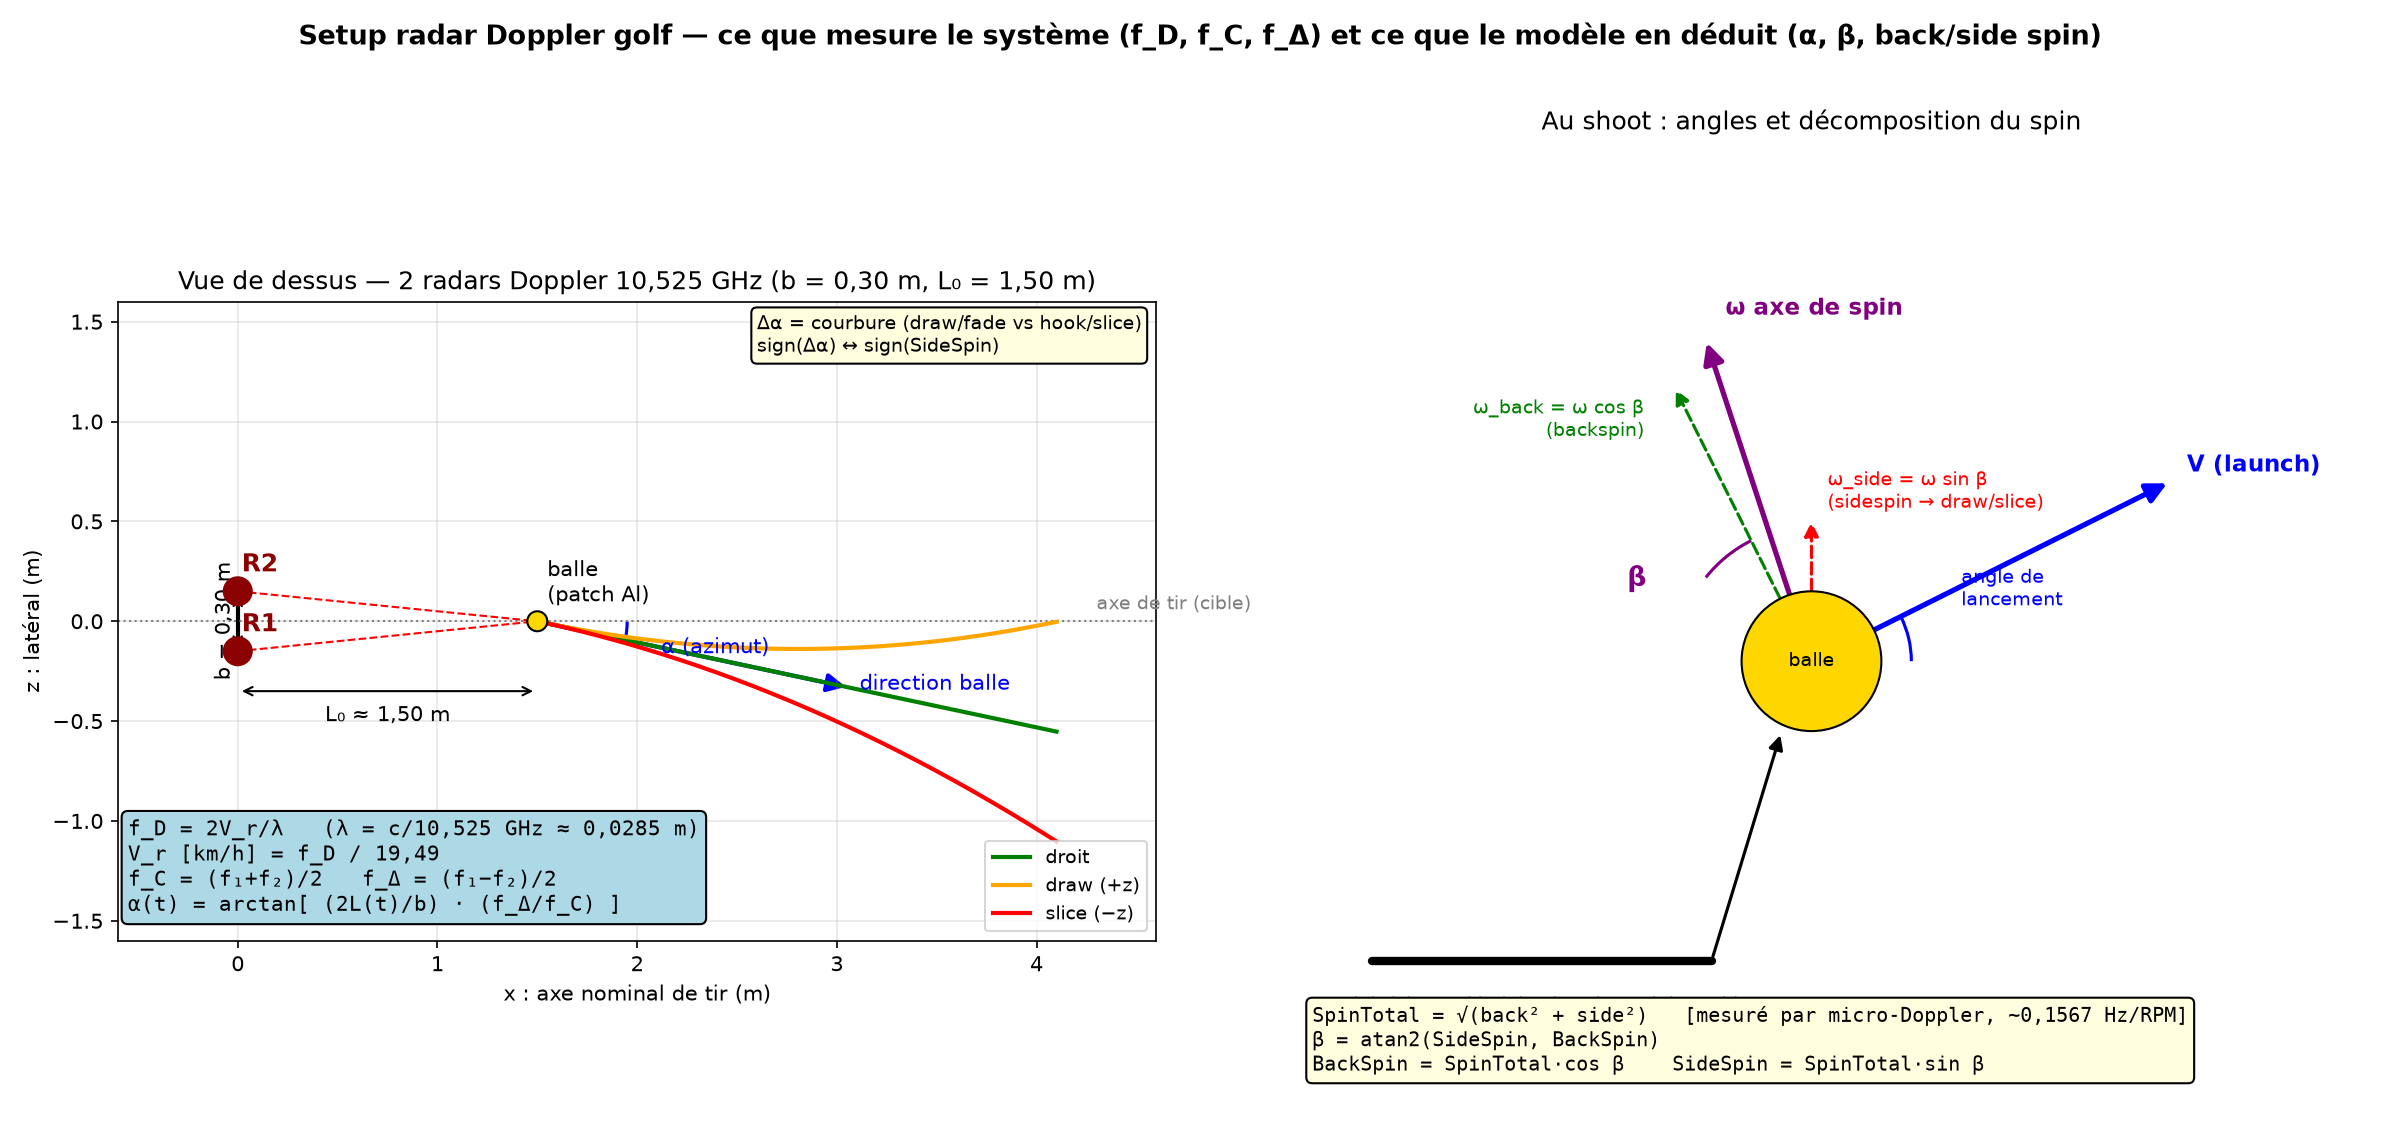
\includegraphics[width=8cm,keepaspectratio]{../sci/img/setup_radar.png}
\caption{Géométrie du dispositif radar (aussi dans le README).}
\label{fig:setupradar}
\end{figure}

\begin{figure}[H]\centering
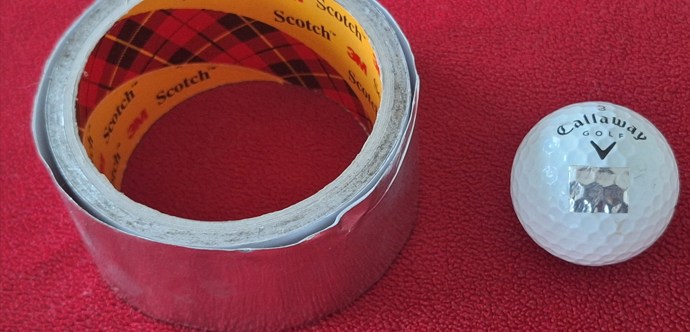
\includegraphics[width=8cm,keepaspectratio]{../sci/img/PatchedBall.png}
\caption{Patch sur la balle (ruban aluminium).}
\label{fig:patchedball}
\end{figure}

\begin{figure}[H]\centering
\includegraphics[width=10cm,keepaspectratio]{../sci/img/spectro\_F7-123m-150kmh-5274trm-210trm-cs111.png}
\caption{Spectrogramme mesuré, coup 123~m / 150~km/h / 5274~tr/min (référence SkyTrak).}
\label{fig:spectro123}
\end{figure}

\begin{figure}[H]\centering
\includegraphics[width=10cm,keepaspectratio]{../sci/img/spectro\_F7-131m-162kmh-6185trm-7102trm-cs124.png}
\caption{Spectrogramme mesuré, coup 131~m / 162~km/h / 6185 back + 7102 latéral tr/min ($\beta\approx48{,}9^\circ$, forte courbure).}
\label{fig:spectro131}
\end{figure}

\begin{figure}[H]\centering
\includegraphics[width=10cm,keepaspectratio]{../sci/img/spectro\_F7-137m-166kmh-4990trm-1312trm-cs118.png}
\caption{Spectrogramme mesuré, coup 137~m / 166~km/h / 4990+1312~tr/min ($\beta\approx14{,}7^\circ$).}
\label{fig:spectro137}
\end{figure}

\begin{figure}[H]\centering
\includegraphics[width=11cm,keepaspectratio]{../sci/img/spectro\_MODELE\_2025-11-08.png}
\caption{Capture théorique (générée), config F7 151~km/h, départ $16{,}5^\circ$, spin 4000~tr/min, latéral 700~tr/min ($\beta=10{,}1^\circ$), club 115~km/h, portée 102~m.}
\label{fig:spectromodele}
\end{figure}

\begin{figure}[H]\centering
\includegraphics[width=11cm,keepaspectratio]{../sci/img/spectro\_MODELE\_102m-151kmh.png}
\caption{Capture générée, même config, version swing complet 450~ms (v2).}
\label{fig:spectromodele102}
\end{figure}

\begin{figure}[H]\centering
\includegraphics[width=11cm,keepaspectratio]{../sci/img/spectro\_MODELE\_137m-166kmh.png}
\caption{Capture générée avec les paramètres du vrai coup de 137~m (166~km/h, 4990/1312~tr/min, club 118).}
\label{fig:spectromodele137}
\end{figure}

\begin{figure}[H]\centering
\includegraphics[width=9cm,keepaspectratio]{../sci/img/traj\_MODELE\_2025-11-08.png}
\caption{Trajectoire modèle (vol + déviation latérale du slice) pour la capture générée du 2025-11-08.}
\label{fig:trajmodele}
\end{figure}

\chapter{Listings}
\section{Golfball.sci}
\begin{lstlisting}[language=matlab, caption=Listing de la simulation de vol de la balle de golf, label={lst:gaolfballsci}]
// Copyright (C) 2016 - Corporation - Author
//
//
// Date of creation: 16 juin 2016
//
//SCI2C: DEFAULT_PRECISION= DOUBLE
//
// ReadWave : FFT_Mat.sce
// 

\end{lstlisting}

\chapter*{}
\section{Remerciements}
Une première version de ce projet a été écrite en 2016 puis laissée de côté. Elle a été reprise en 2026 à la lumière de la puissance des outils d'IA. J'ai repris le projet pour évaluer et apprendre à utiliser l'IA : trouver des bugs dans le code Scilab historique, porter la chaîne de traitement en Python et améliorer les estimateurs au fil de nos discussions (médiane post-impact robuste plutôt que le max global, périodicité du patch plutôt que l'excursion spectrale seule, appariement stéréo des deux radars, contrôles qualité). Cela a aussi montré que le montage électronique (deux radars Doppler 10,525~GHz, amplificateur, Arduino Nano, carte son USB) était bien faisable et cohérent. La traduction française de ce document a été entièrement réalisée par une IA (Mistral Vibe).

\section*{Conflits d'intérêts}
Les auteurs déclarent n'avoir aucun conflit d'intérêts.

\bibliographystyle{alpha}
\selectlanguage{french}
\bibliography{biblioBibTex}
%\end{multicols}\newpage



%\input{PageEnd.tex}
\end{document}
